%%%%%%%%%%%%%%%%%%%%%%%%%%%%%%%%%%%%%%%%%%%%%%%%%%%%%%%%%%%%%%%%%%%%%%%
\documentclass[t]{beamer}
\usetheme{metropolis}

\usepackage{enumitem}
\usepackage{animate}
\usepackage{svg}
\usepackage{bbding,pifont}
\usepackage{minted}
\usepackage{xcolor}
\usepackage{pdfpages}
\usepackage{listings}
\usepackage{hyperref}

\usepackage{tikz}
\usetikzlibrary{intersections}
\usetikzlibrary{shapes.geometric, arrows,positioning}

\usepackage[edges]{forest}
\hypersetup{
    colorlinks=true,
    linkcolor=blue,
    filecolor=magenta,
    urlcolor=cyan,
}

\urlstyle{same}


\usepackage{etoolbox}
\AtBeginDocument{%
  \renewcommand{\normalsize}{\small}
  \renewcommand{\small}{\footnotesize}
  \renewcommand{\footnotesize}{\scriptsize}
}

\makeatletter
\patchcmd{\minted@pygmentize}
  {\minted@addto@extra{\minted@opt{fontsize}}}
  {\minted@addto@extra{\minted@opt{fontsize}=\\scriptsize}}
  {}{}
\makeatother

\definecolor{exampletitle}{RGB}{0,102,204} % Custom title background
\definecolor{examplebg}{RGB}{230,230,230} % Light gray body background

\setbeamercolor{block title example}{fg=white, bg=exampletitle}
\setbeamercolor{block body example}{fg=black, bg=examplebg}

\newenvironment{customexampleblock}[1]{
    \begin{center}
        \begin{beamercolorbox}[wd=\textwidth, sep=0.05em, rounded=true, center]{block title example}
            \makebox[\textwidth][c]{\textbf{#1}}
        \end{beamercolorbox}
        \begin{beamercolorbox}[wd=\textwidth, sep=0.05em, rounded=true, center]{block body example}
}{
        \end{beamercolorbox}
    \end{center}
}

\renewcommand{\normalsize}{\fontsize{9pt}{11pt}\selectfont}


%% setup complete
\begin{document}

%%%%%%%%%%%%%%%%%%%%%%%%%%%%%%%%%%%%%%%%%%%%%%%%%%%%%%%%%%%%%%%%%%%%%%%%%%%%%%%
%% Title Slide
\title{
    PyVista for CAE Datasets: \\
    Streamlining 3D Visualization and Analysis
}

\author{
{\large Alex Kaszynski} \\[4pt]
{\large Bane Sullivan} \\[4pt]
{\large Tetsuo Koyama} \\[4pt]
{\large And \href{https://github.com/pyvista/pyvista/graphs/contributors}{180+ GitHub Contributors}}
}

\date{
\vspace{20pt}
{\large Advanced Modeling \& Simulation (AMS) Seminar Series} \\[6pt]
{\large NASA Ames Research Center} \\[12pt]
{\large \today}
}

\maketitle

%%%%%%%%%%%%%%%%%%%%%%%%%%%%%%%%%%%%%%%%%%%%%%%%%%%%%%%%%%%%%%%%%%%%%%%%%%%%%%%
\begin{frame}{Table of Contents}
    \tableofcontents
\end{frame}

\begin{frame}{Speaker: Alex Kaszynski}

    \begin{columns}
        \begin{column}{0.3\textwidth}
            \centering
            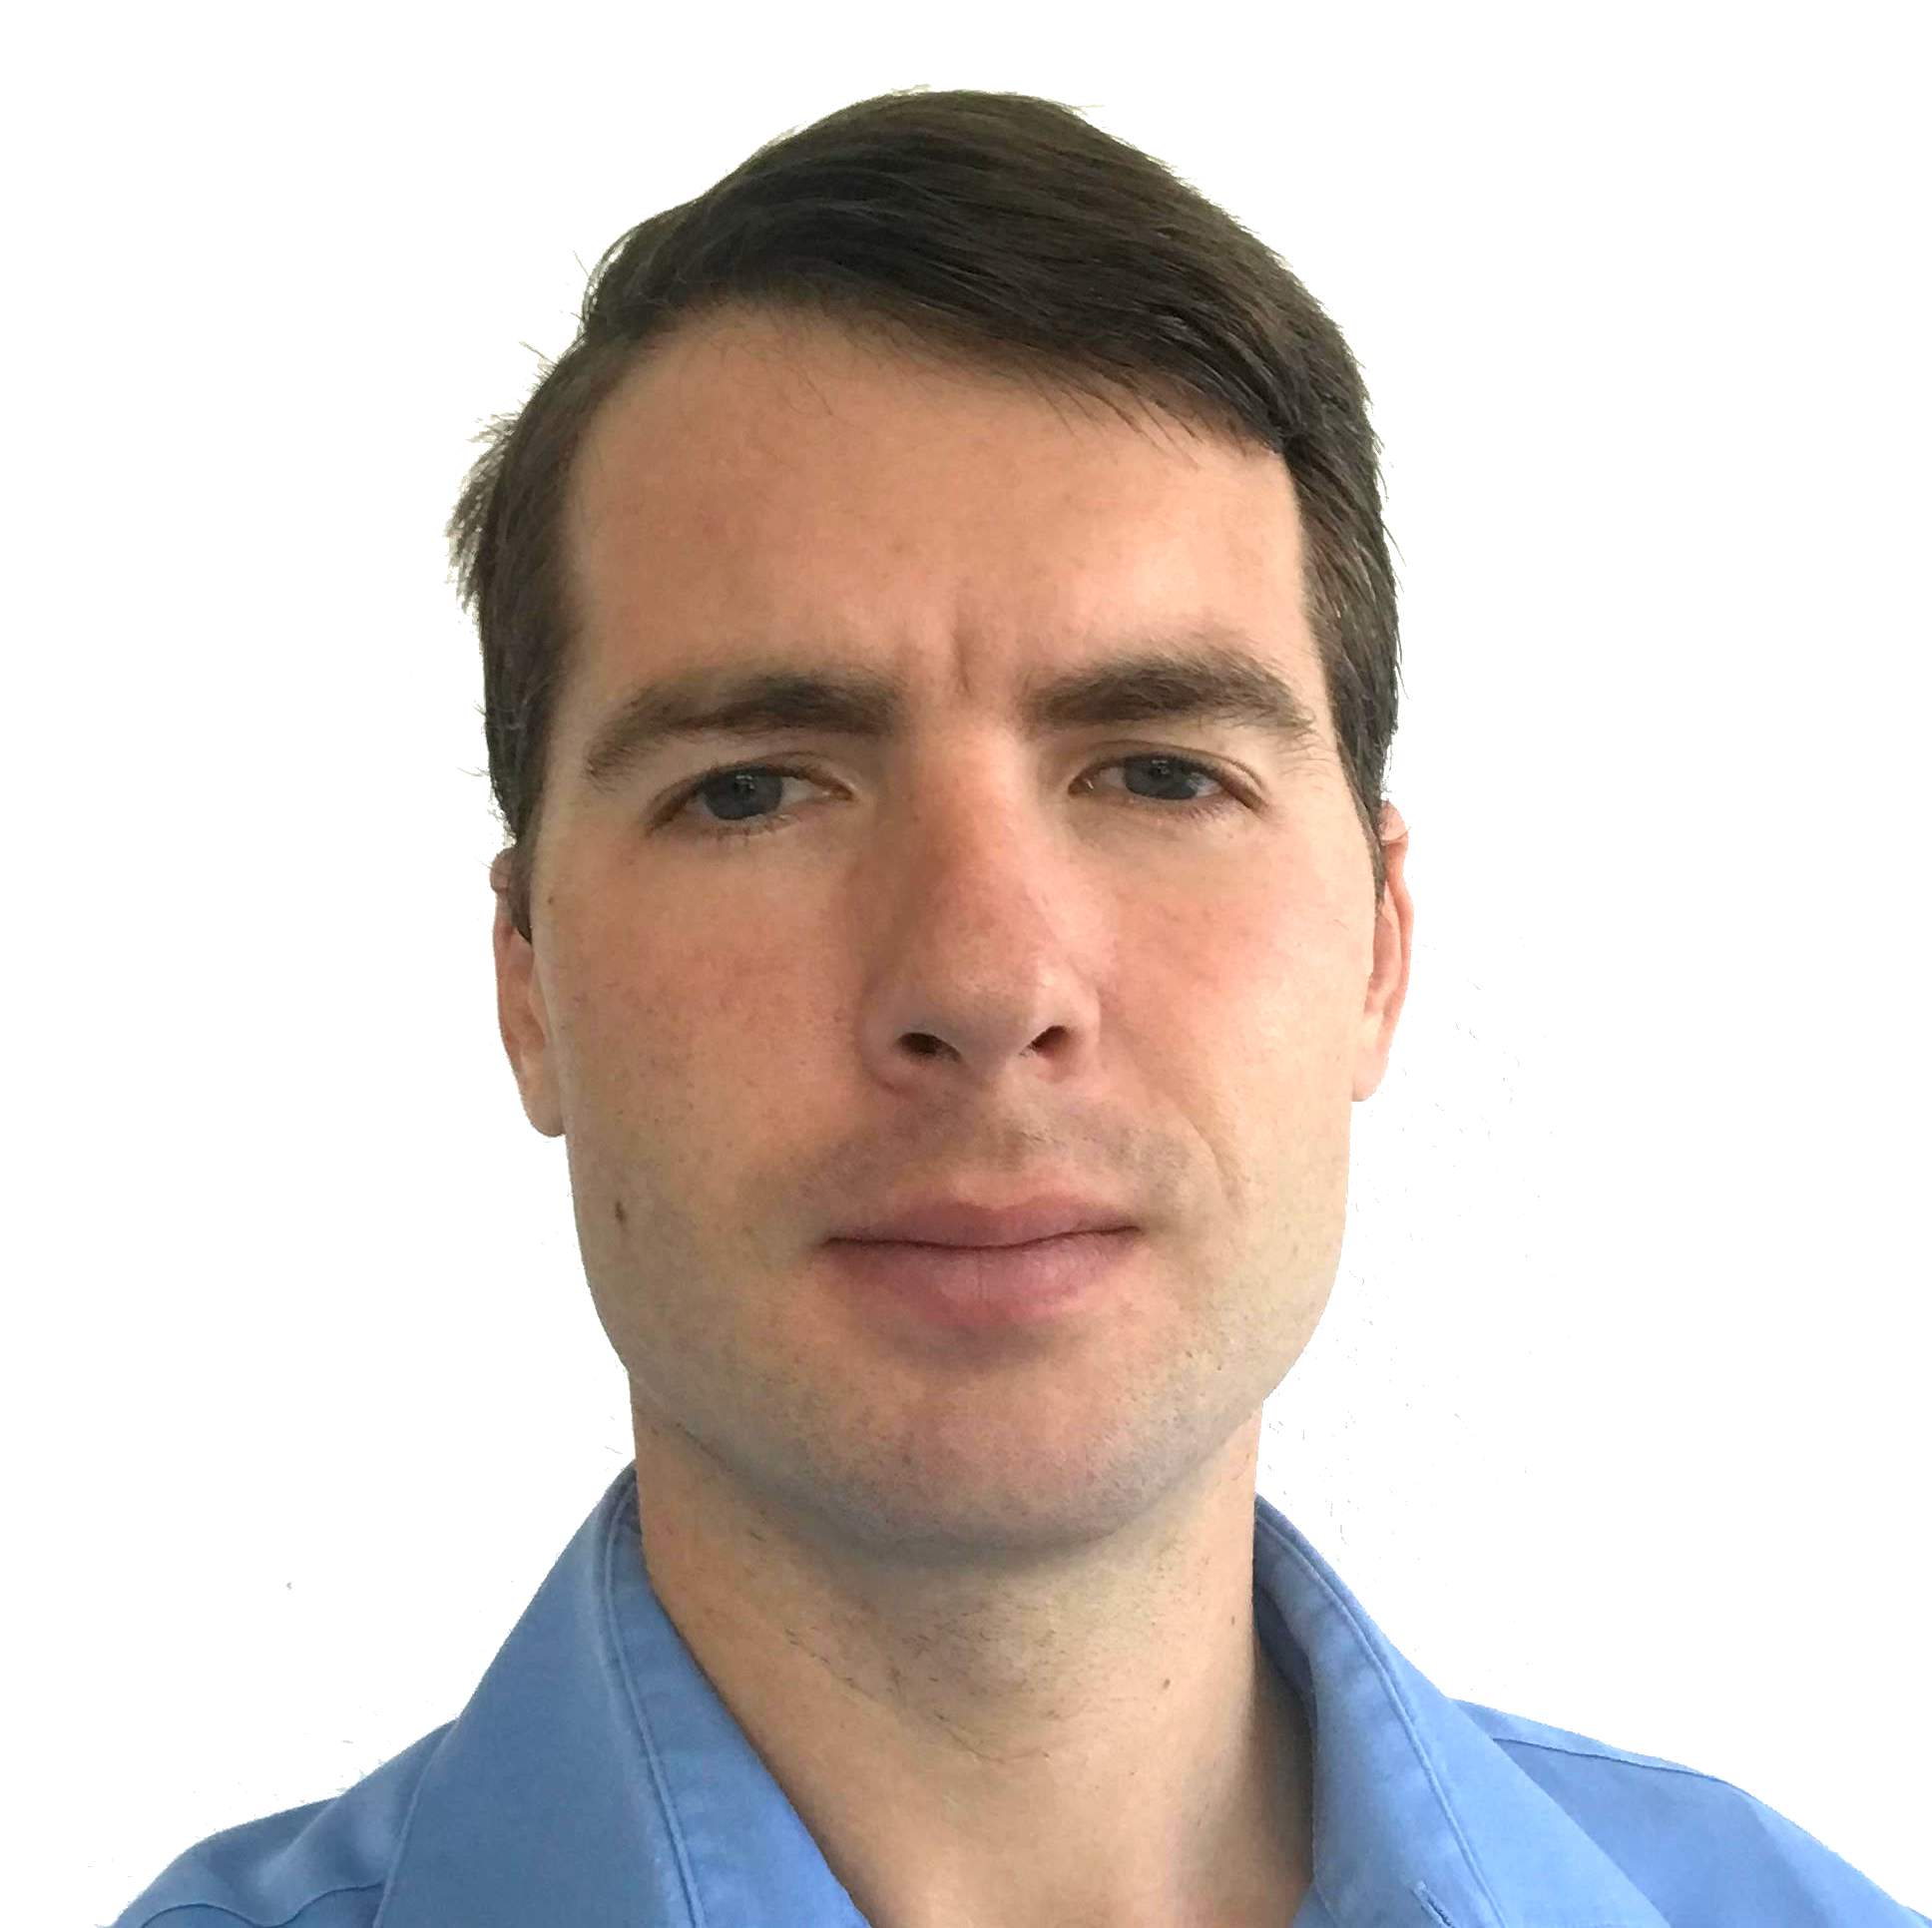
\includegraphics[width=0.8\textwidth]{figures/alex-kaszynski-trans.png}\\[40pt]
            
\includegraphics[width=1.0\textwidth]{figures/afrl-logo.png} \\[40pt]
            
\includegraphics[width=1.0\textwidth]{figures/Pasteur.png}
        \end{column}
        \begin{column}{0.7\textwidth}
            \textbf{Staff Simulation Engineer, Pasteur ISI \& AFRL/USAF}
            \begin{itemize}[leftmargin=10pt, label=•]
                \item Co-creator of \textbf{PyVista}, an open-source Python library for 3D visualization and mesh analysis.
                \item Former Distinguished Engineer at \textbf{Ansys} and creator of PyAnsys, a suite of Python libraries to interface with Ansys's products.
                \item Advocate for open-source tools in research, engineering, and scientific computing.
                \item Extensive experience in computational engineering, scientific visualization, and CAE workflows.
            \end{itemize}
        \end{column}
    \end{columns}

\end{frame}

%%%%%%%%%%%%%%%%%%%%%%%%%%%%%%%%%%%%%%%%%%%%%%%%%%%%%%%%%%%%%%%%%%%%%%%%%%%%%%%
\section{PyVista - Introduction}

\begin{frame}
    \frametitle{VTK: A Powerful and Widely Adopted Visualization Toolkit}

    \centering
    \Large
    \textbf{The Backbone of Scientific Visualization} \\[10pt]

    \normalsize
    \textbf{Key Statistics and Adoption:} \\[10pt]

    \begin{itemize}[leftmargin=10pt, label=•]
        \item \textbf{Established in 1993}, VTK has over 5 million lines of code, reflecting its extensive development.
        \item \textbf{2.5+ million downloads annually} from Kitware’s servers.
        \item \textbf{Global research adoption}: Over 100 papers per year in China since 2007 in medical imaging, geological exploration, and aerospace.
        \item \textbf{Foundation for major applications}: Powers ParaView, \href{https://en.wikipedia.org/wiki/VisIt}{VisIt}, and many other industry-standard tools.
        \item \textbf{Designed for modern computing}: Supports GPU acceleration and fine-grained parallelism through VTK-m.
    \end{itemize}

    \vspace{10pt}
    \textbf{Sources:} \href{https://www.kitware.com/happy-birthday-vtk-30-years-of-innovation/}{Kitware}, \href{https://www.exascaleproject.org/highlight/ecp-brings-much-needed-visualization-software-to-exascale-and-gpu-accelerated-systems/}{Exascale Project}

\end{frame}

%%%%%%%%%%%%%%%%%%%%%%%%%%%%%%%%%%%%%%%%%%%%%%%%%%%%%%%%%%%%%%%%%%%%%%%%%%%%%%%
\subsection{Comparison - VTK vs. PyVista}

\begin{frame}
    \frametitle{Comparison - VTK vs. PyVista}

    \vspace{15pt}

    \begin{columns}[T]
        \begin{column}{.5\textwidth}
            \textbf{Raw VTK Implementation} \\[5pt]
            \inputminted[fontsize=\tiny]{python}{code/vtk_example.py}
        \end{column}

        \begin{column}{.5\textwidth}
            \textbf{Simplified PyVista Approach} \\[5pt]
            \inputminted[fontsize=\tiny]{python}{code/pv_example.py}
            \begin{center}
                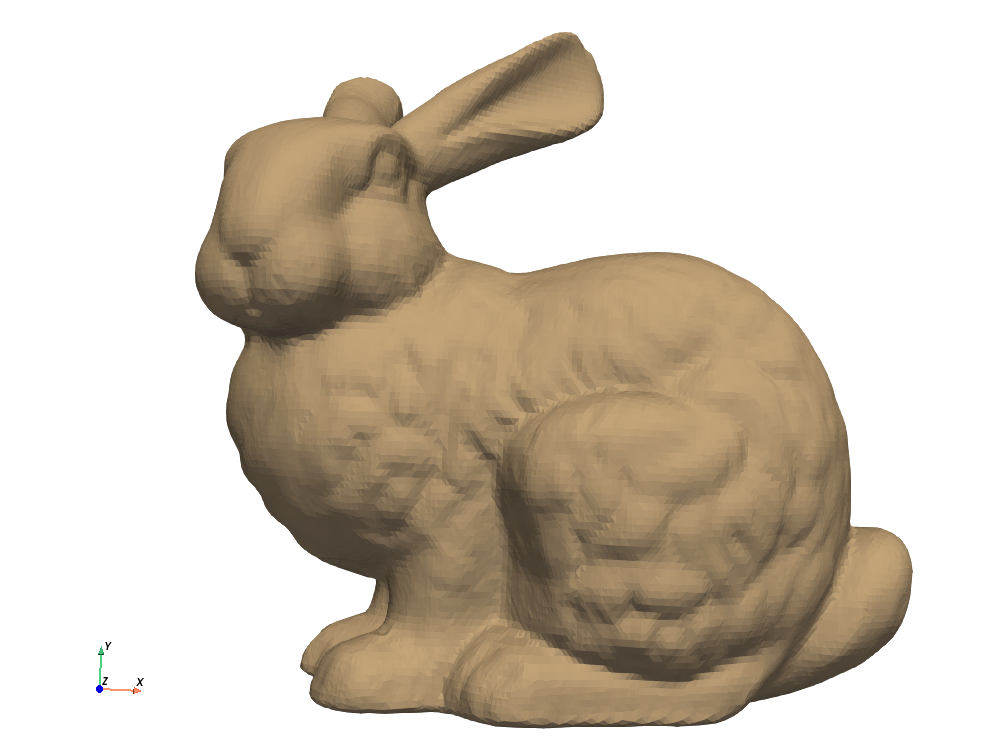
\includegraphics[width=0.9\textwidth]{figures/pv_example_trans.png}
            \end{center}
        \end{column}
    \end{columns}

    \vspace{15pt}

    Follow along with our online docs at \href{https://dev.pyvista.org/getting-started/why}{Plotting a Mesh using PyVista}.

\end{frame}

%%%%%%%%%%%%%%%%%%%%%%%%%%%%%%%%%%%%%%%%%%%%%%%%%%%%%%%%%%%%%%%%%%%%%%%%%%%%%%%
\begin{frame}
    \frametitle{The Philosophy Behind PyVista}

    \begin{customexampleblock}{Guiding Principles}
        \begin{itemize}[leftmargin=10pt, label=\ding{51}]
            \vspace{-5pt}
            \item Enable Python developers to work naturally within their ecosystem.
            \item Reduce boilerplate without sacrificing power or flexibility.
            \item Provide immediate, intuitive access to visualization and mesh operations.
        \end{itemize}
    \end{customexampleblock}

    %% \vspace{5pt}
    %% \textbf{Core Tenets of PyVista}

    \begin{itemize}[leftmargin=10pt, label=\ding{228}]
        \item \textbf{Minimalism}: Less code. PyVista wraps complex VTK functionality into concise, readable syntax.
        \item \textbf{Documentation and Examples}: Classes and methods are meticulously documented with interactive examples.
        \item \textbf{Integration with Python Ecosystem}: Native integration with NumPy and other scientific libraries for intuitive data inspection and manipulation.
        \item \textbf{Automatic Resource Management}: Handles object lifecycle, memory, and cleanups internally.
    \end{itemize}

    %% \vspace{5pt}
    \centering
    \textbf{PyVista is built for Python developers who expect their data visualization tools to look and operate just like the rest of their data science libraries.}

\end{frame}

%%%%%%%%%%%%%%%%%%%%%%%%%%%%%%%%%%%%%%%%%%%%%%%%%%%%%%%%%%%%%%%%%%%%%%%%%%%%%%%
\begin{frame}
    \frametitle{PyVista - Library Origin}
    Originally designed to replace repetitive boiler plate code within the mesh metamorphosis application \href{https://www.femorph.com/}{FEMORPH}. Open sourced in 2016 and developed over 8 years of community involvement and 180+ contributors.
    \vspace{-5pt}
    \begin{center}
        \setlength{\fboxrule}{0.5pt}
        \setlength{\fboxsep}{0pt}
        \fcolorbox{black}{white}{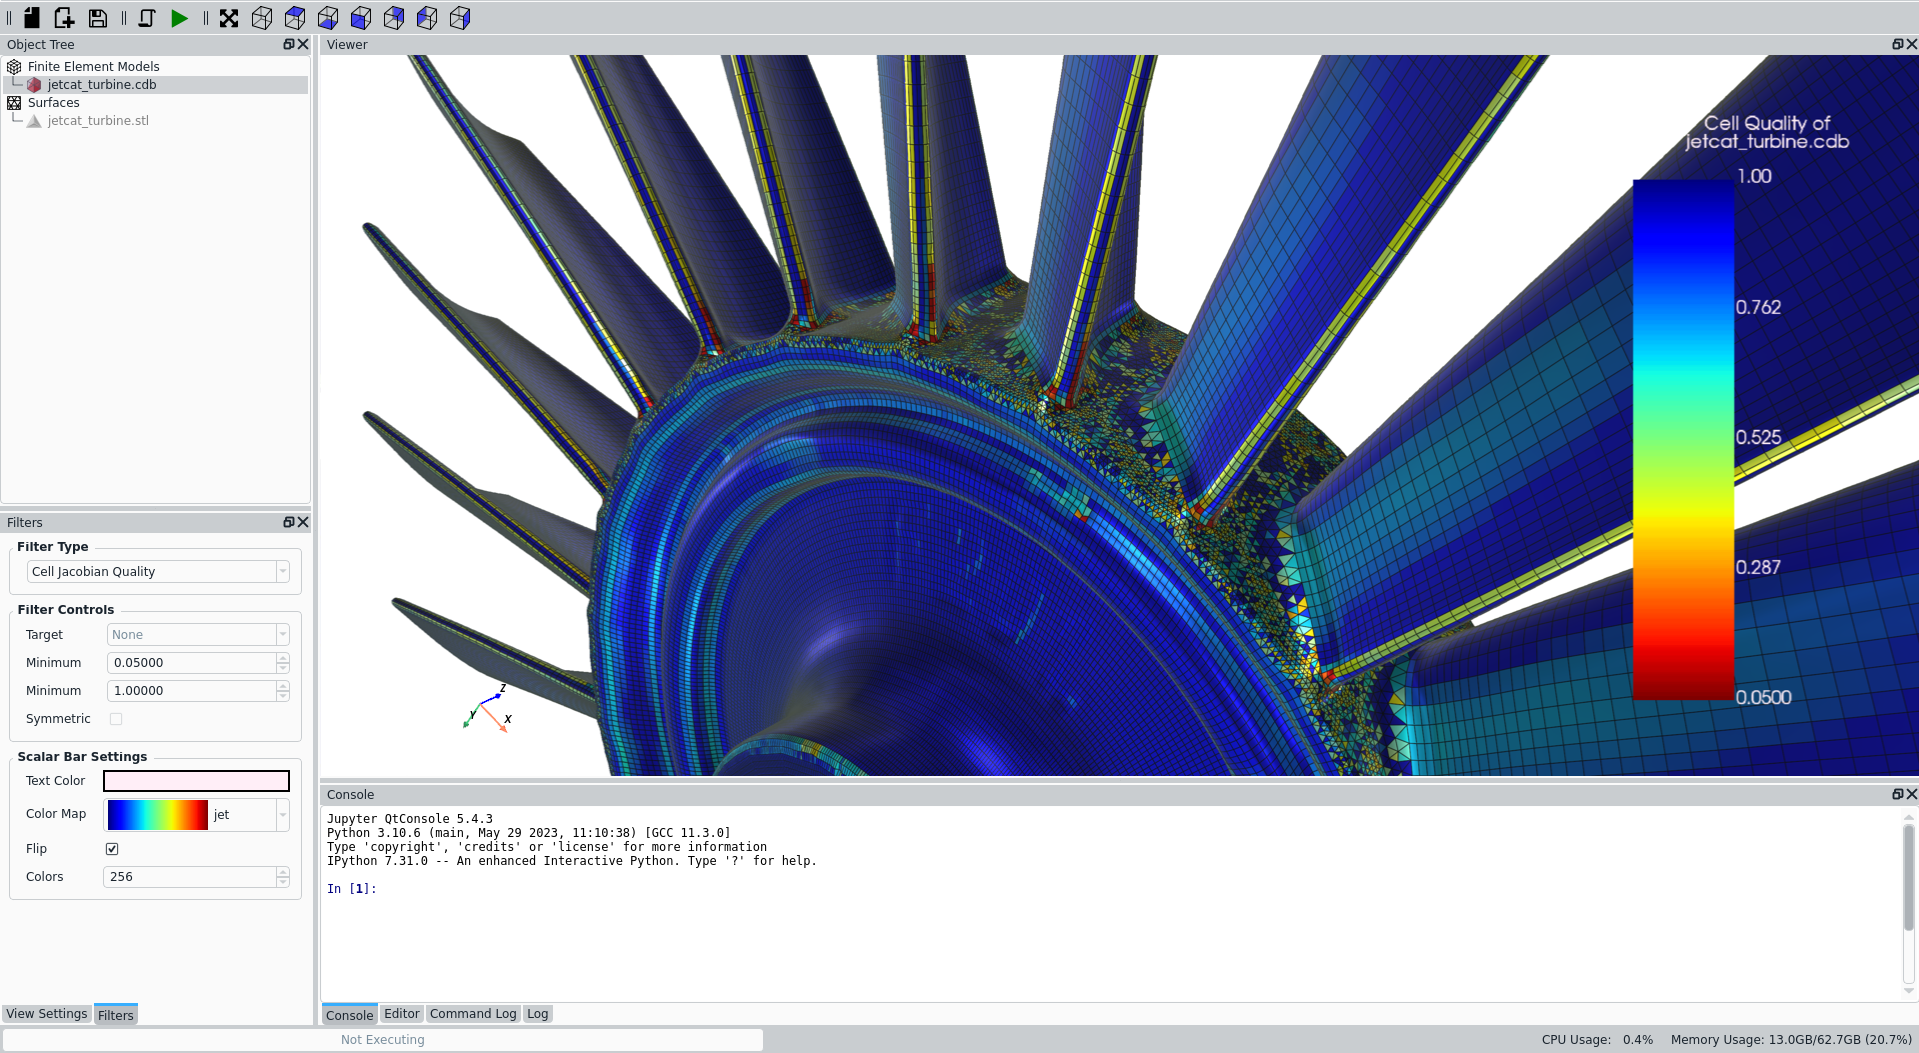
\includegraphics[width=1.0\textwidth]{figures/femorph-latest.png}}
    \end{center}
\end{frame}

%% %%%%%%%%%%%%%%%%%%%%%%%%%%%%%%%%%%%%%%%%%%%%%%%%%%%%%%%%%%%%%%%%%%%%%%%%%%%%%%%
%% \begin{frame}
%%     \frametitle{PyVista - Brief History}

%%     \begin{itemize}[leftmargin=8pt, label=•]
%%         \item Created as a library for \href{https://www.wpafb.af.mil/News/Article-Display/Article/1503043/afrl-signs-first-of-its-kind-software-license-with-pratt-whitney/}{femorph} by \href{https://github.com/akaszynski}{@akaszynski} in 2016
%%         \item Posted to GitHub as \href{https://github.com/akaszynski/vtki}{akaszynski/vtki} in 2017
%%         \item Vastly expanded by (co-founder) \href{https://github.com/banesullivan/}{@banesullivan} in 2018
%%         \item First release of \href{https://pypi.org/project/pyvista/#history}{PyVista} on PyPI in 2019
%%         \item Published a paper \href{https://joss.theoj.org/papers/10.21105/joss.01450}{PyVista: 3D plotting and mesh analysis through a streamlined interface for VTK} in late 2019
%%         \item As of March 2025, over 180 contributors and \href{https://github.com/pyvista/pyvista/stargazers}{3k Stars} on GitHub with over 4000 PRs merged
%%         \item Used by at least 3.8k other GitHub repositories
%%         \item Greatly expanded community presence and continuing support thanks to:
%%               \begin{itemize}[leftmargin=10pt, label=•]
%%                   \item \href{https://github.com/tkoyama010}{@tkoyama010 (Tetsuo Koyama)}
%%                   \item \href{https://github.com/adeak}{@adeak}
%%                   \item \href{https://github.com/MatthewFlamm}{@MatthewFlamm}
%%                   \item \href{https://github.com/user27182}{@user27182}
%%                   \item \href{https://github.com/pyvista/pyvista/graphs/contributors}{And many others}
%%               \end{itemize}
%%     \end{itemize}
%% \end{frame}

%%%%%%%%%%%%%%%%%%%%%%%%%%%%%%%%%%%%%%%%%%%%%%%%%%%%%%%%%%%%%%%%%%%%%%%%%%%%%%%
\begin{frame}
    \frametitle{PyVista - Popularity and Growth}

    \begin{center}
        \begin{columns}[T]
            \begin{column}{.6\textwidth}
                \small
                \begin{itemize}[leftmargin=10pt, label=•]
                    \item Already the most popular 3D visualization library on PyPI.
                    \item Designed not just for visualization, but for scientific
                          visualization focused on data post-processing, file IO, and
                          interoperability with other libraries.
                    \item Supports a growing ecosystem with strong community
                          contributions and integrates with tools like \texttt{Jupyter},
                          \texttt{VTK}, and \texttt{meshio}.
                \end{itemize}
            \end{column}

            \begin{column}{.5\textwidth}
                \vspace{-5pt}
                \centering
                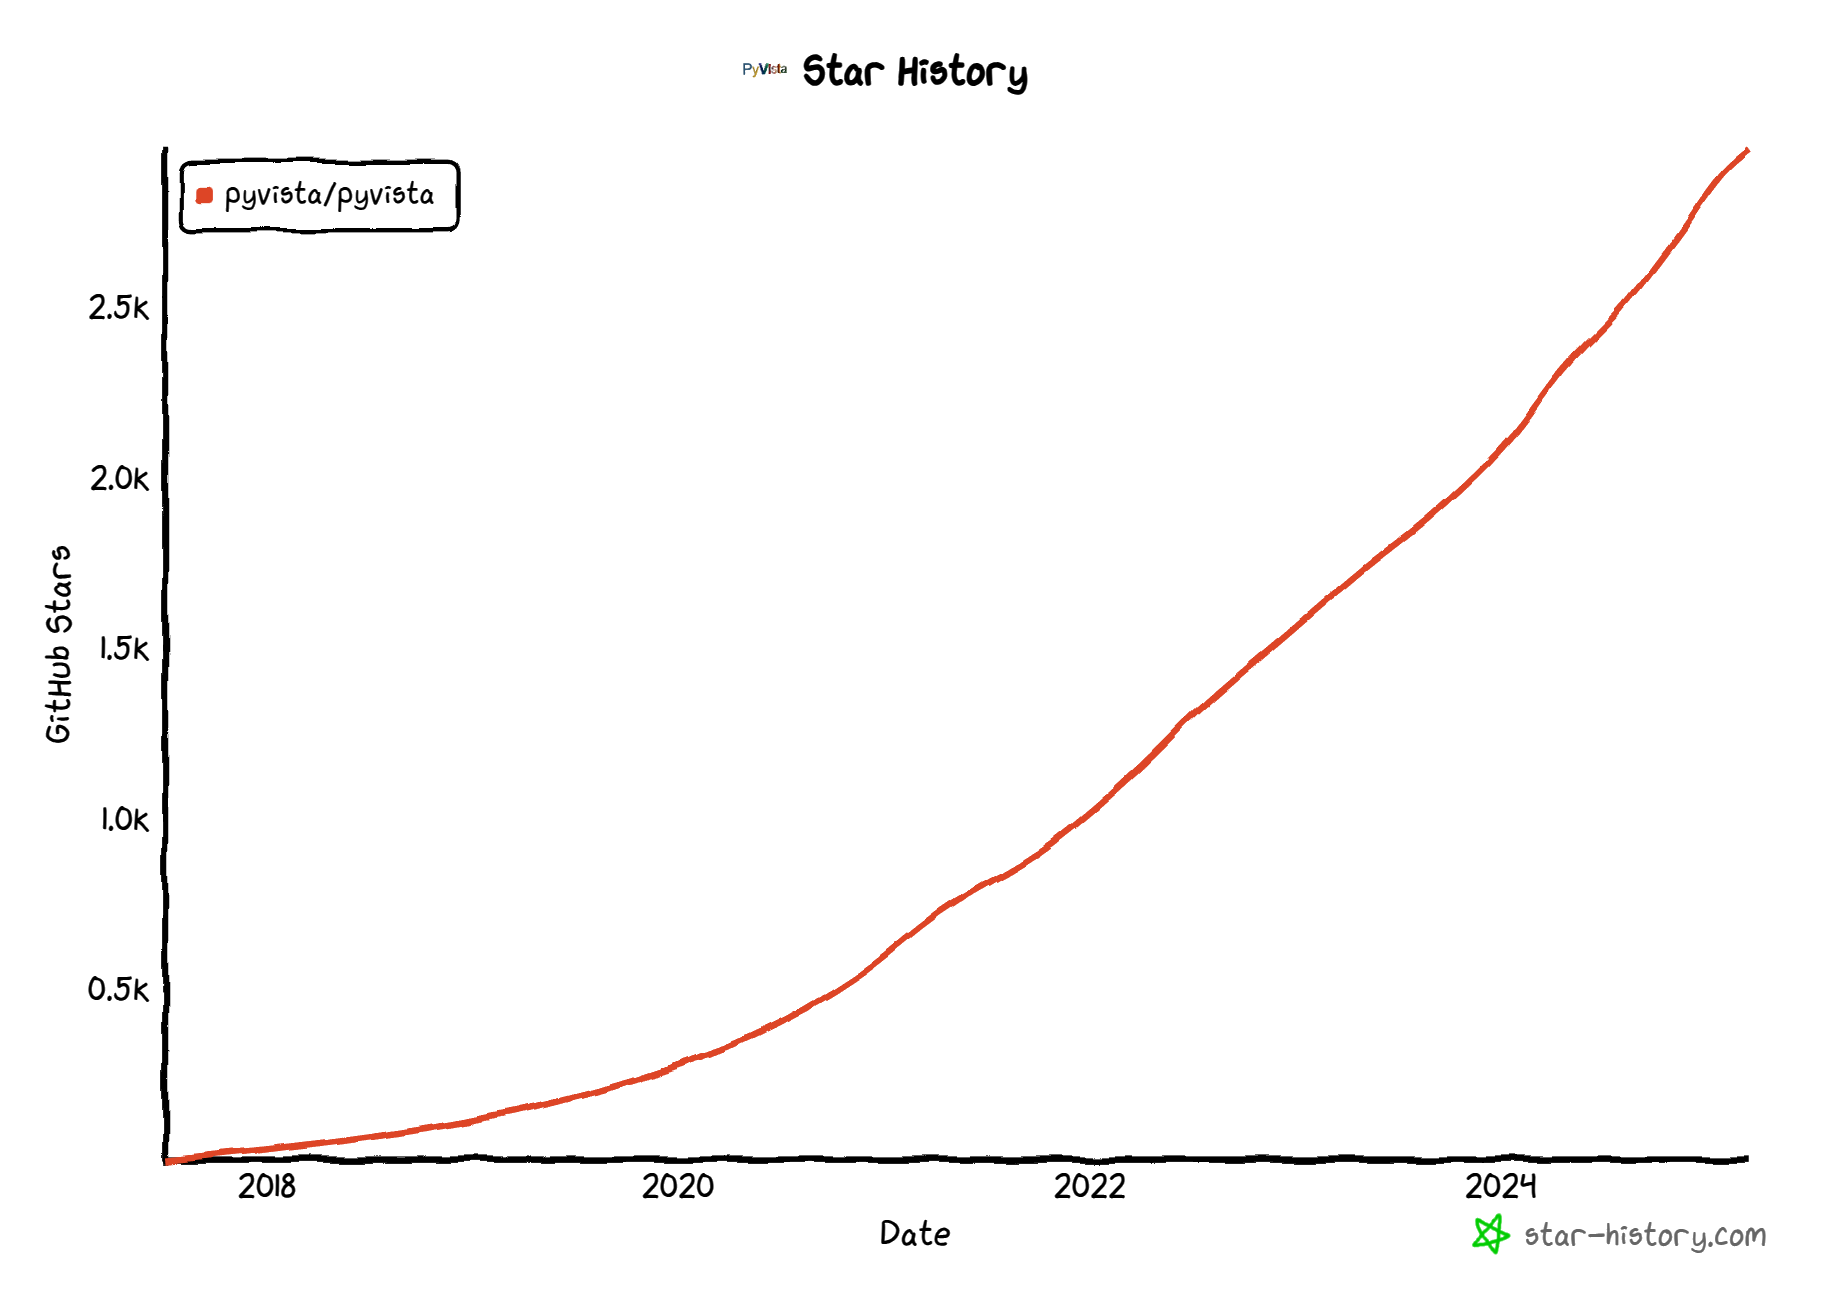
\includegraphics[width=0.9\textwidth]{figures/overview-stars-graph-trans.png}
            \end{column}

        \end{columns}

        \vspace{10pt}
        \href{https://pyviz.org/tools.html}{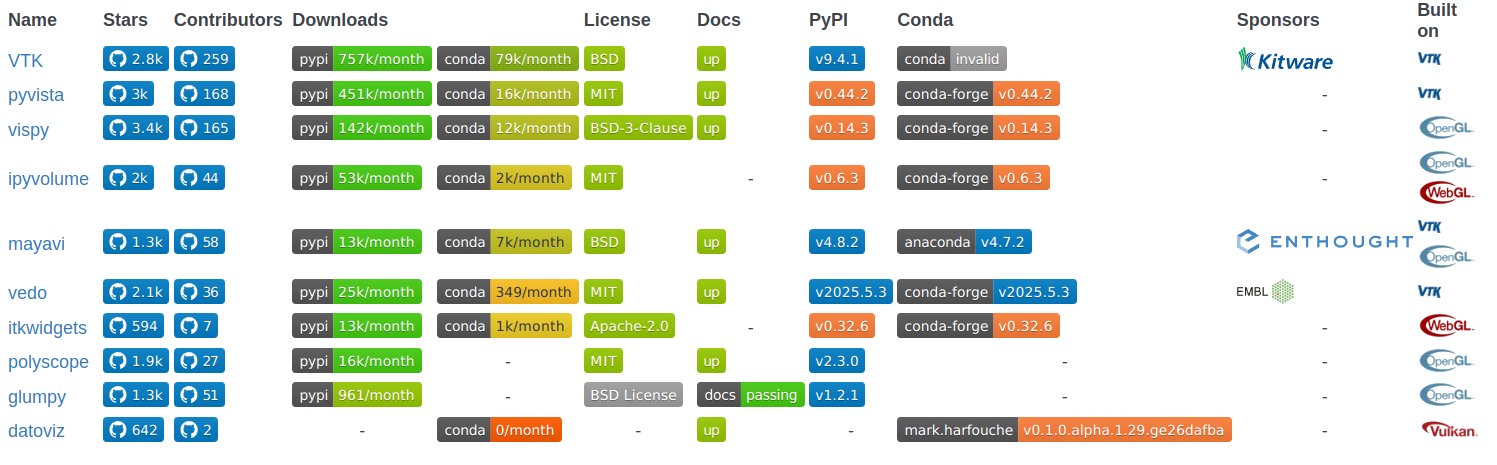
\includegraphics[width=1.0\textwidth]{figures/overview_sciviz_trans.png}}

    \end{center}

\end{frame}

%%%%%%%%%%%%%%%%%%%%%%%%%%%%%%%%%%%%%%%%%%%%%%%%%%%%%%%%%%%%%%%%%%%%%%%%%%%%%%%
\begin{frame}
    \frametitle{PyVista - Libraries Showcase}

    Several open-source CAE projects that leverage PyVista

    \vspace{-5pt}

    \begin{columns}[T]
        \begin{column}{.25\textwidth}
            \begin{customexampleblock}{\small AeroSandbox}
                \centering
                \begin{minipage}[c][2cm][c]{\textwidth}
                    \href{https://github.com/peterdsharpe/AeroSandbox}{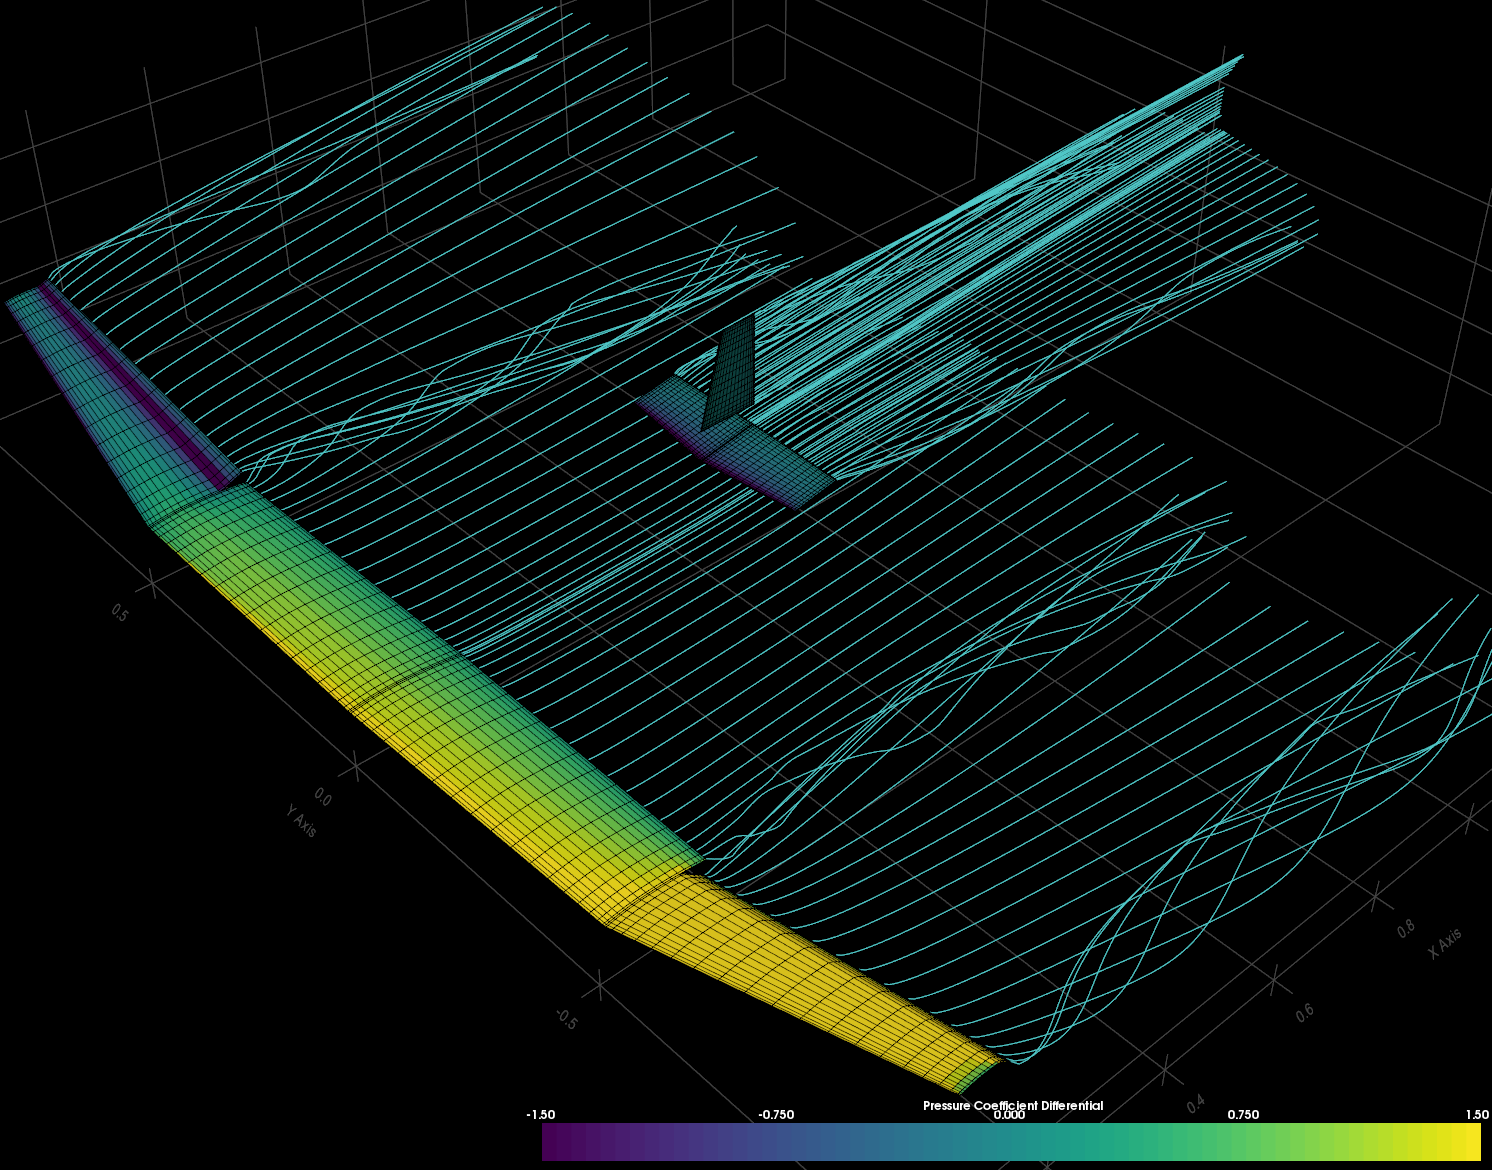
\includegraphics[width=\textwidth,height=3.5cm,keepaspectratio]{figures/aerosandbox.png}}
                \end{minipage}
            \end{customexampleblock}
        \end{column}

        \begin{column}{.25\textwidth}
            \begin{customexampleblock}{\small Felupe}
                \centering
                \begin{minipage}[c][2cm][c]{\textwidth}
                    \href{https://felupe.readthedocs.io/en/stable/examples/index.html}{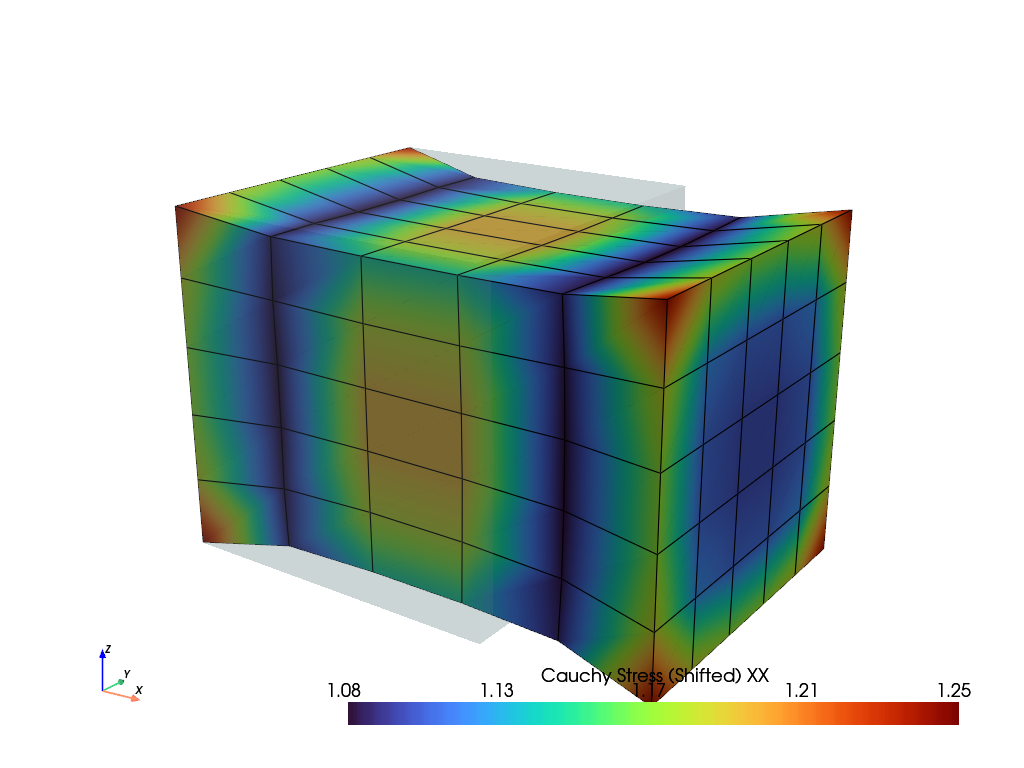
\includegraphics[width=\textwidth,height=3.5cm,keepaspectratio]{figures/felupe.png}}
                \end{minipage}
            \end{customexampleblock}
        \end{column}

        \begin{column}{.25\textwidth}
            \begin{customexampleblock}{\small PteraSoftware}
                \centering
                \begin{minipage}[c][2cm][c]{\textwidth}
                    \href{https://github.com/camUrban/PteraSoftware}{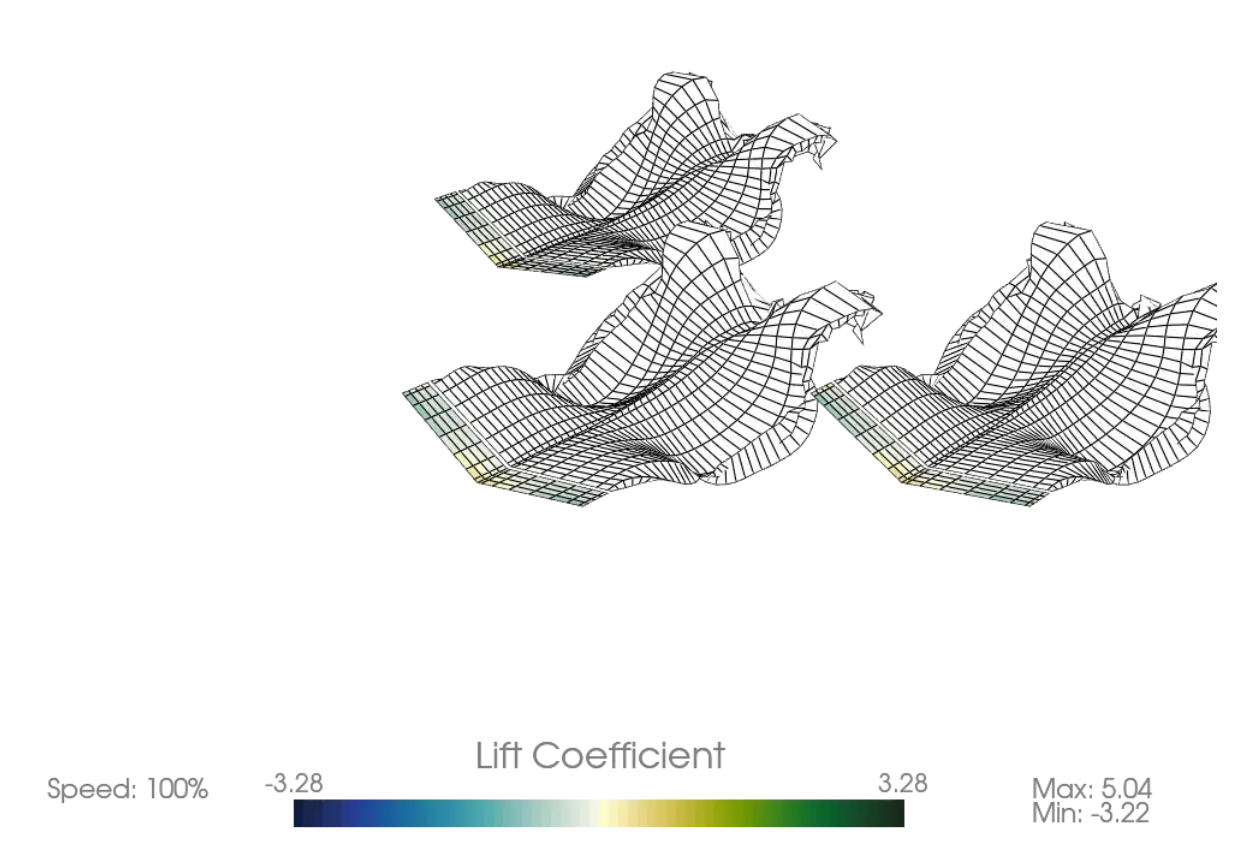
\includegraphics[width=\textwidth,height=3.5cm,keepaspectratio]{figures/ptera.png}}
                \end{minipage}
            \end{customexampleblock}
        \end{column}

        \begin{column}{.25\textwidth}
            \begin{customexampleblock}{\small Magpylib}
                \centering
                \begin{minipage}[c][2cm][c]{\textwidth}
                    \href{https://magpylib.readthedocs.io/en/latest/index.html}{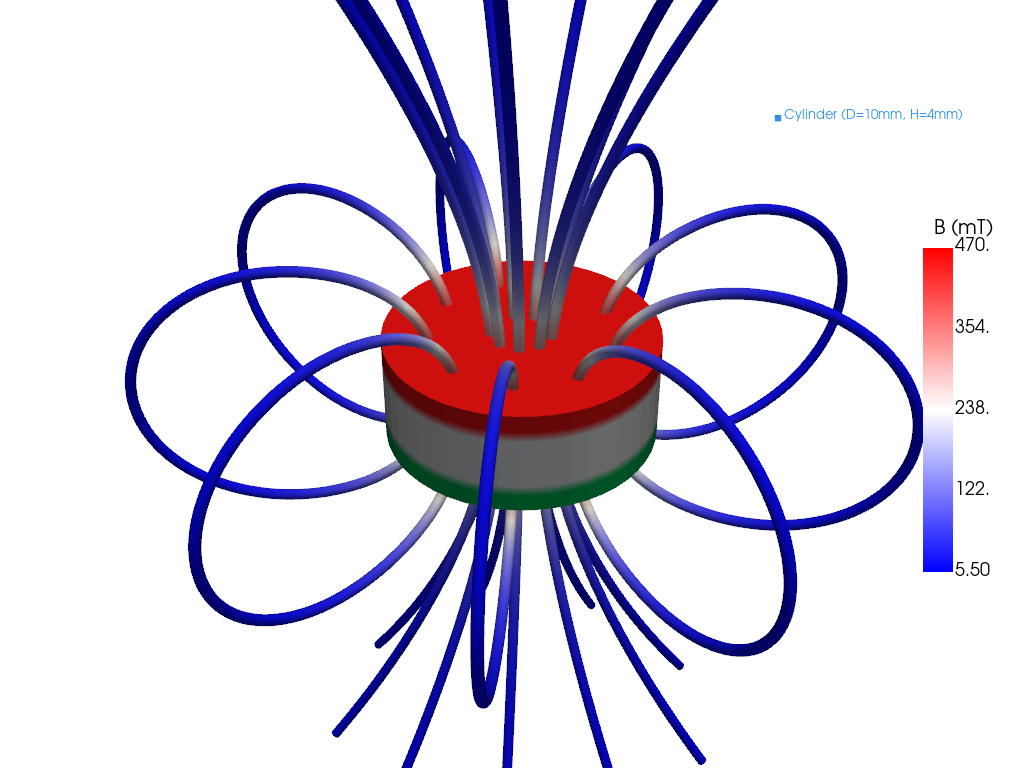
\includegraphics[width=\textwidth,height=3.5cm,keepaspectratio]{figures/magpylib.png}}
                \end{minipage}
            \end{customexampleblock}
        \end{column}
    \end{columns}

    \vspace{-5pt}

    \begin{columns}[T]
        \begin{column}{.25\textwidth}
            \begin{customexampleblock}{\small PyMAPDL}
                \centering
                \href{https://mapdl.docs.pyansys.com/}{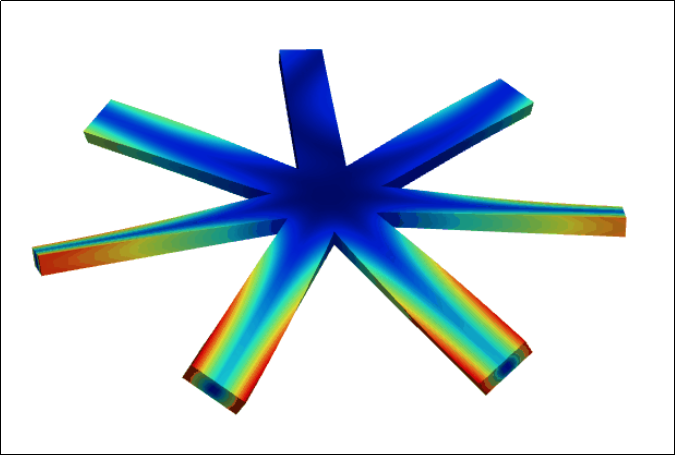
\includegraphics[width=\textwidth,height=3.5cm,keepaspectratio]{figures/pymapdl_eo_disc.png}}
            \end{customexampleblock}
        \end{column}

        \begin{column}{.25\textwidth}
            \begin{customexampleblock}{\small dolfinx}
                \centering
                \href{https://docs.fenicsproject.org/dolfinx/main/python/demos/demo_pyvista.html}{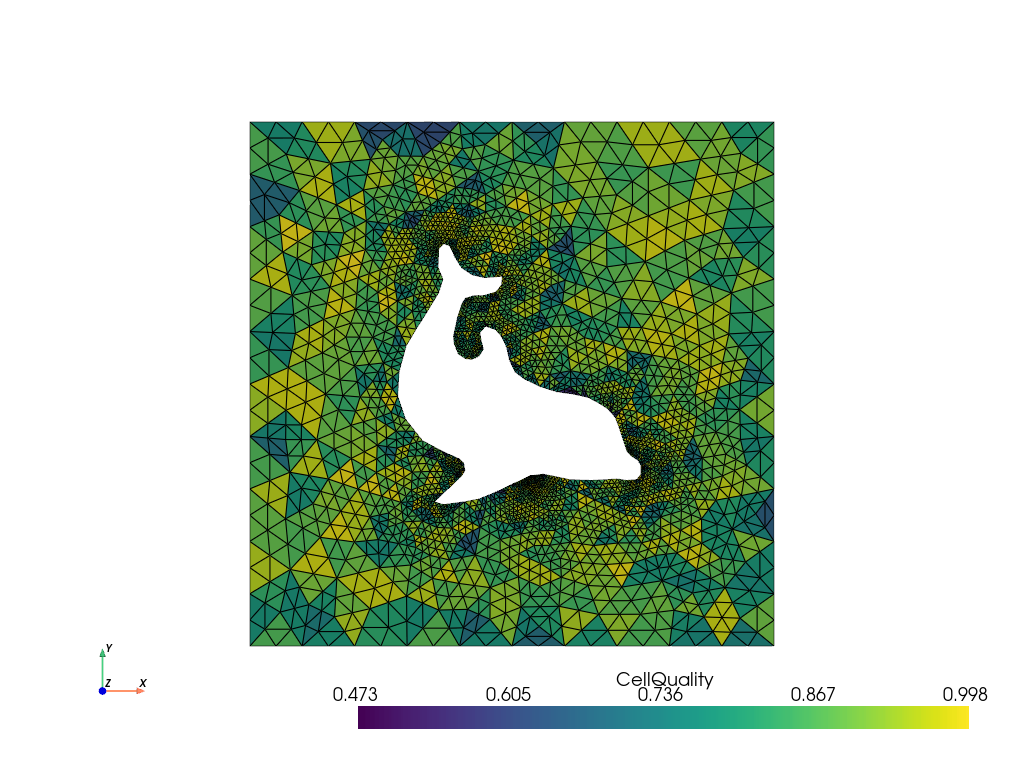
\includegraphics[width=\textwidth,height=3.5cm,keepaspectratio]{figures/dolfinx.png}}
            \end{customexampleblock}
        \end{column}

        \begin{column}{.25\textwidth}
            \begin{customexampleblock}{\small Pyleecan}
                \centering
                \href{https://www.pyleecan.org/gallery.html}{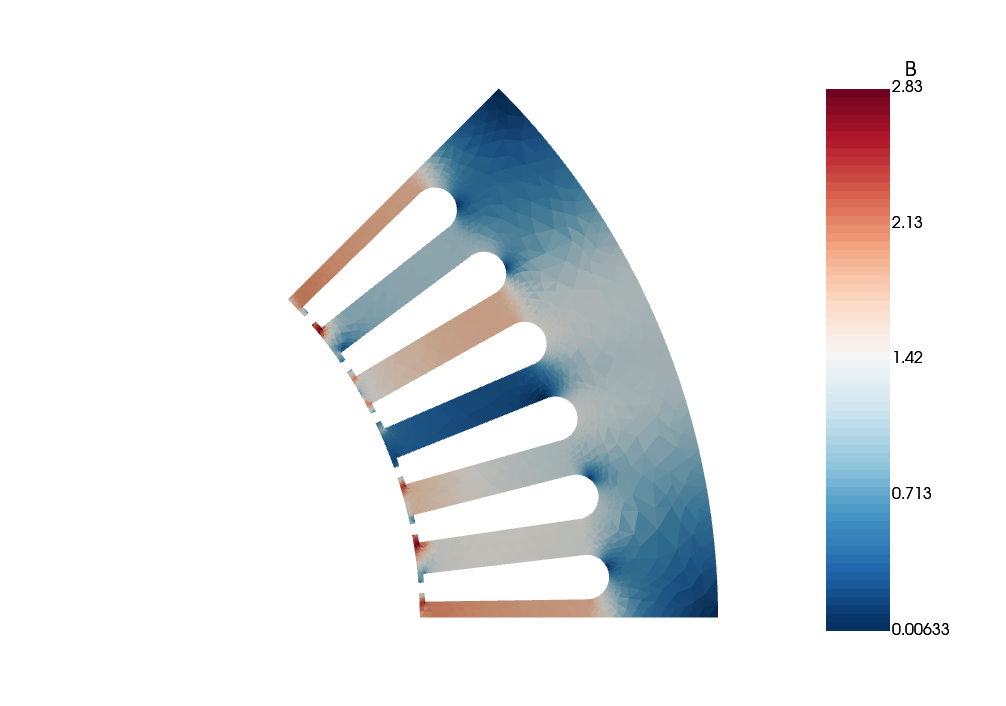
\includegraphics[width=\textwidth,height=3.5cm,keepaspectratio]{figures/pyleecan.png}}
            \end{customexampleblock}
        \end{column}

        \begin{column}{.25\textwidth}
            \begin{customexampleblock}{\small MNE }
                \centering
                \href{https://github.com/mne-tools/mne-python}{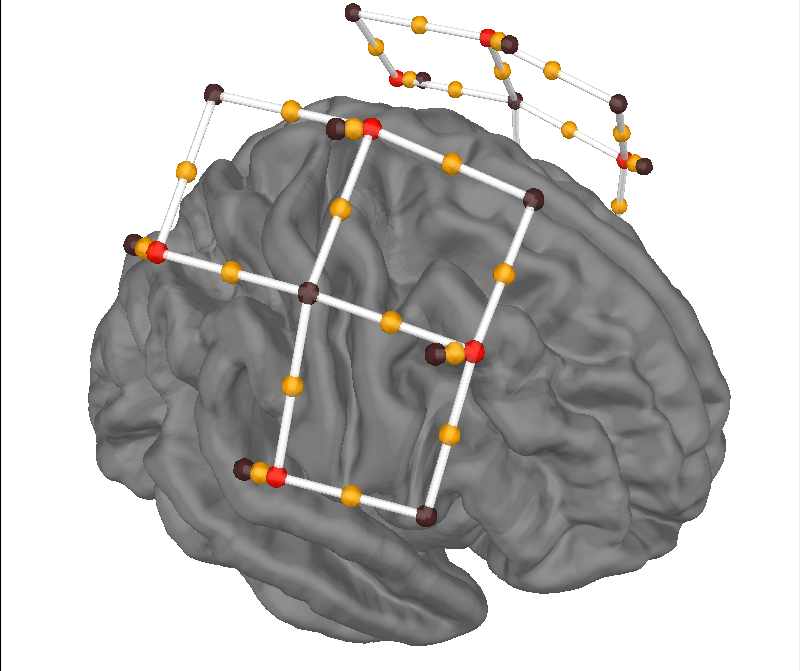
\includegraphics[width=\textwidth,height=3.5cm,keepaspectratio]{figures/mne.png}}
            \end{customexampleblock}
        \end{column}
    \end{columns}

    \vspace{1cm}
    \centering
    And many \href{https://docs.pyvista.org/getting-started/connections}{more}!

\end{frame}

%%%%%%%%%%%%%%%%%%%%%%%%%%%%%%%%%%%%%%%%%%%%%%%%%%%%%%%%%%%%%%%%%%%%%%%%%%%%%%%
\begin{frame}

    \frametitle{Incorporating PyVista within a CAE Workflow or Application}

    \begin{center}
        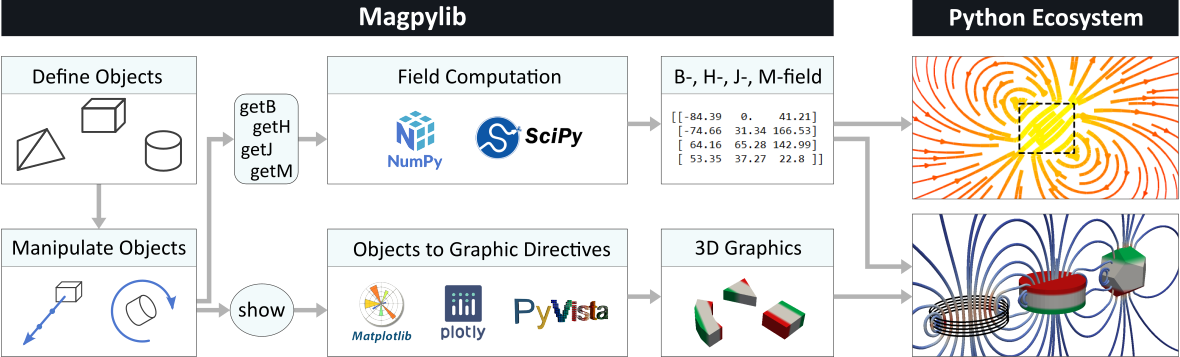
\includegraphics[width=1.0\textwidth]{figures/flowchart.png}
    \end{center}

    \vspace{-12pt}

    \begin{columns}[T]
        \begin{column}{.3\textwidth}
            \begin{customexampleblock}{\small Viewer and Data science}
                \centering
                \begin{minipage}[c][3cm][c]{\textwidth}
                    \href{https://discourse.vtk.org/t/pyvista-trame-jupyter-3d-visualization/10610/6}{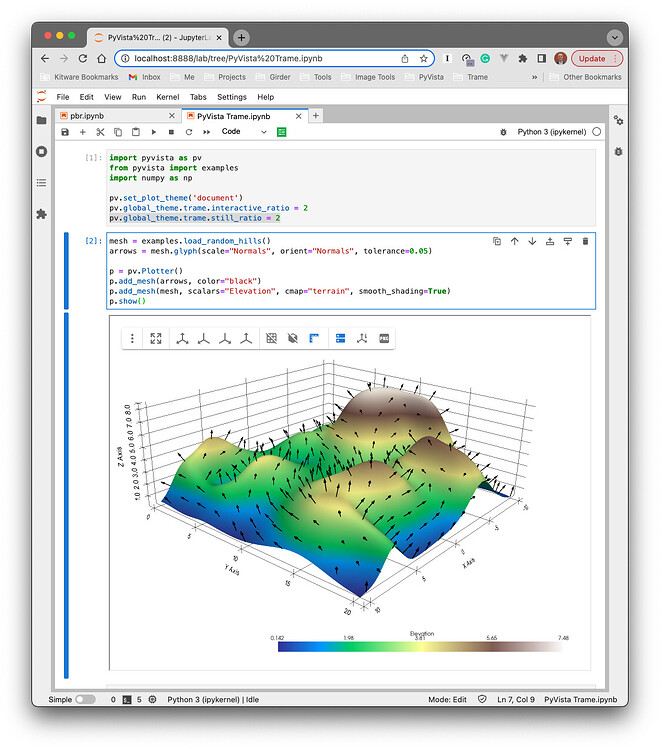
\includegraphics[width=\textwidth,height=3.5cm,keepaspectratio]{figures/jupyterlab.jpeg}}

                \end{minipage}
            \end{customexampleblock}
        \end{column}

        \begin{column}{.3\textwidth}
            \begin{customexampleblock}{\small Library or Standalone Tool}
                \centering
                \begin{minipage}[c][3cm][c]{\textwidth}
                    \href{https://panel-example-production.up.railway.app/}{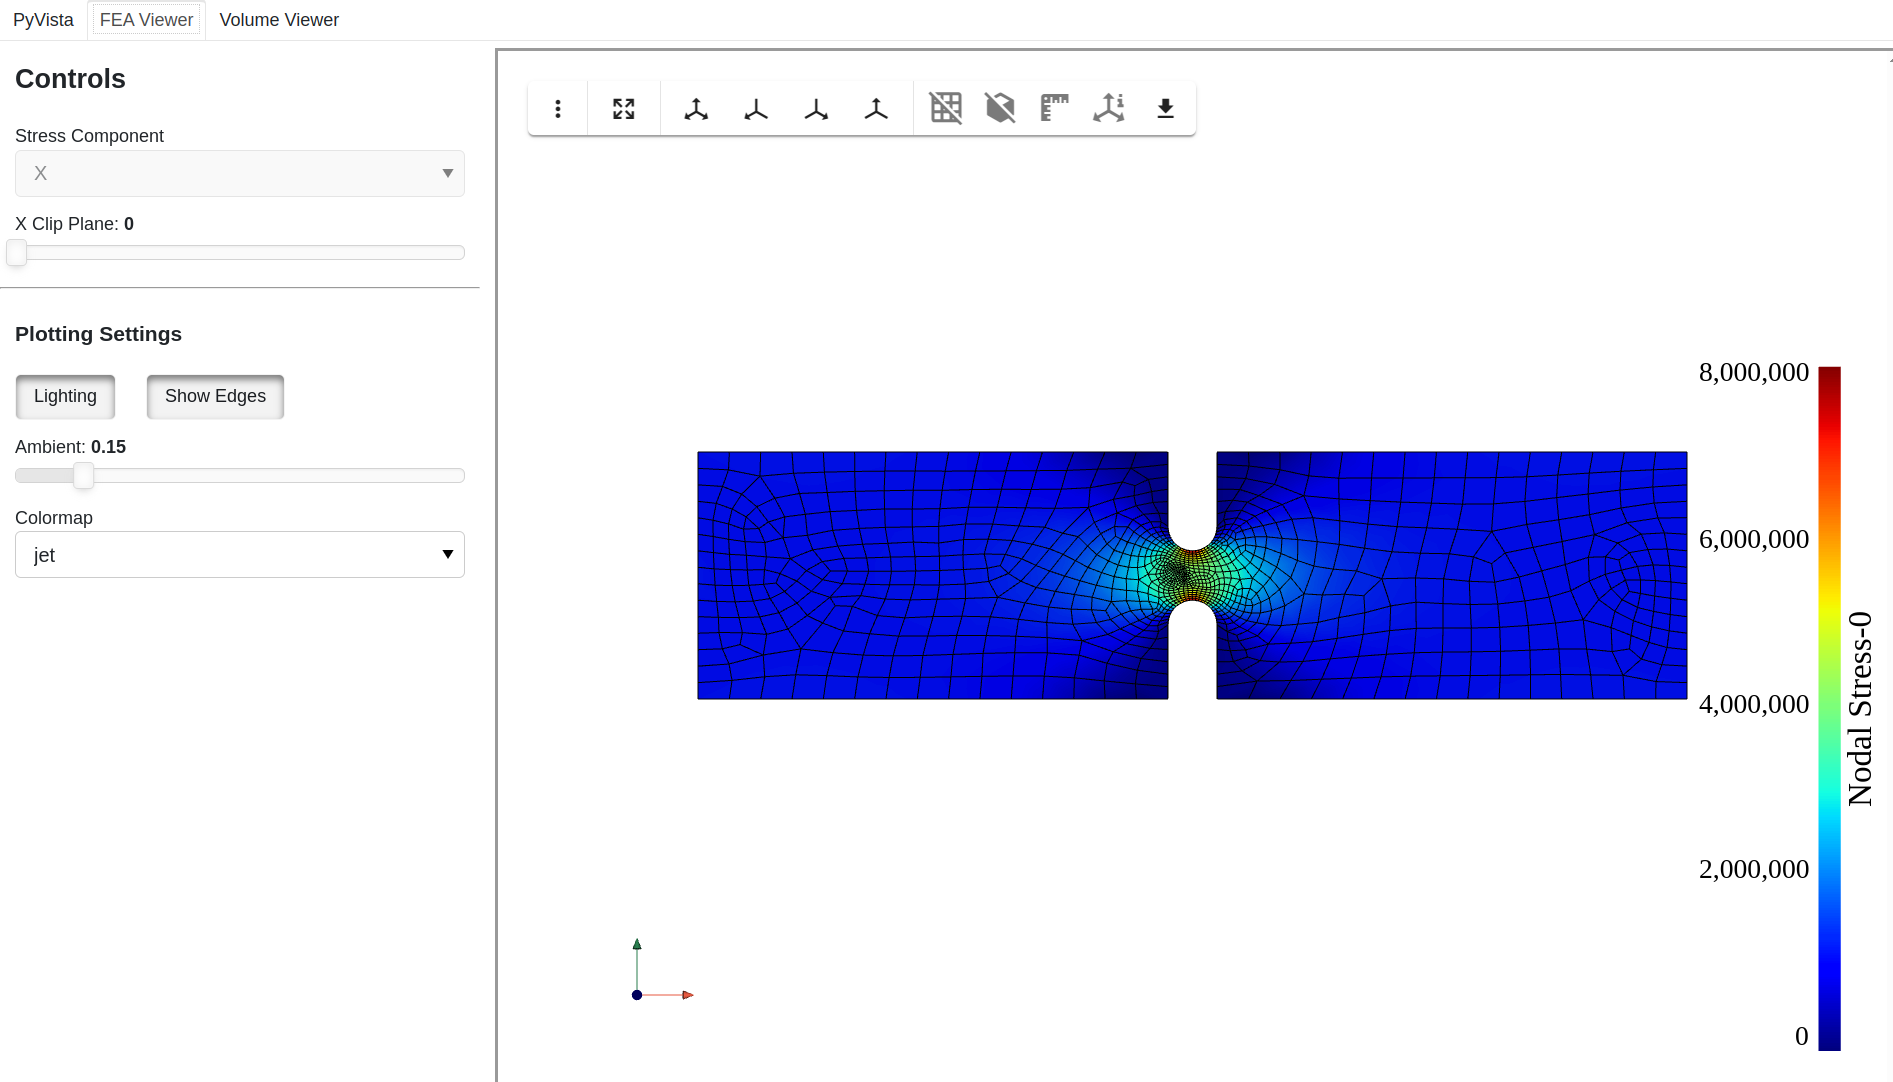
\includegraphics[width=\textwidth,height=3.5cm,keepaspectratio]{figures/panel-pyvista.png}}
                \end{minipage}
            \end{customexampleblock}
        \end{column}

        \begin{column}{.3\textwidth}
            \begin{customexampleblock}{\small Complex Application}
                \centering
                \begin{minipage}[c][3cm][c]{\textwidth}
                    \href{https://www.femorph.com/}{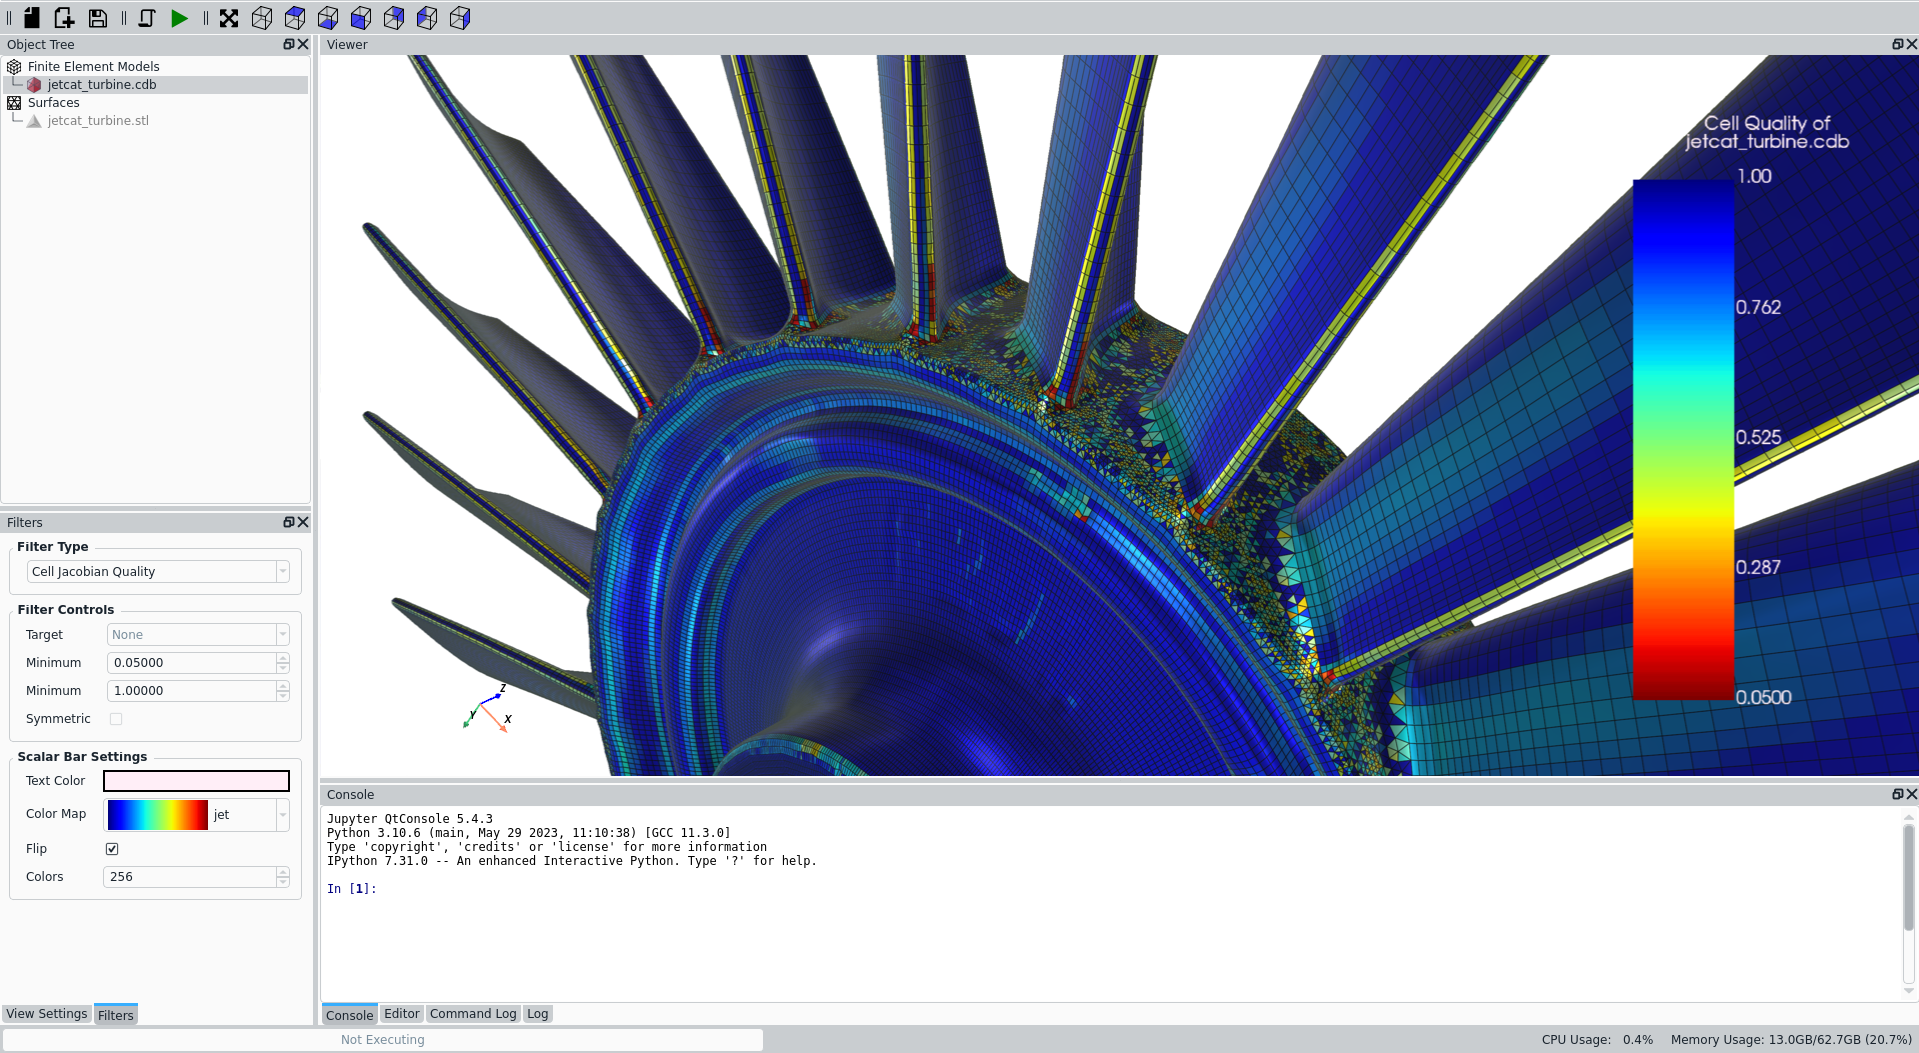
\includegraphics[width=\textwidth,height=3.5cm,keepaspectratio]{figures/femorph-latest.png}}
                \end{minipage}
            \end{customexampleblock}
        \end{column}
    \end{columns}

\end{frame}

%%%%%%%%%%%%%%%%%%%%%%%%%%%%%%%%%%%%%%%%%%%%%%%%%%%%%%%%%%%%%%%%%%%%%%%%%%%%%%%
\begin{frame}{Standing on the Shoulders of Giants}

    \centering
    \textbf{\Large PyVista is built on a foundation of powerful open-source tools}

    \vspace{20pt}

    \begin{columns}[c]
        \begin{column}{0.5\textwidth}
            \begin{itemize}[leftmargin=10pt, label=•]
                \item \textbf{NumPy} – Fundamental package for scientific computing with Python
                \item \textbf{VTK} – Advanced 3D visualization and data processing
                \item \textbf{trame} – Client and Server-side rendering of VTK objects
                \item \textbf{Matplotlib} – Colormaps and 2D plotting
                \item \textbf{Jupyter} – Interactive computing and in-browser computing
            \end{itemize}
        \end{column}

        \begin{column}{0.5\textwidth}
            \centering
            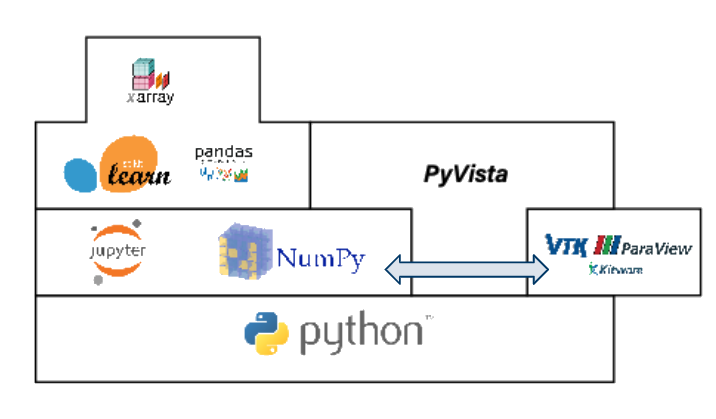
\includegraphics[width=1.0\textwidth]{figures/pyvista_dependencies_trans.png}
        \end{column}
    \end{columns}

    %% \vspace{10pt}

\end{frame}

%%%%%%%%%%%%%%%%%%%%%%%%%%%%%%%%%%%%%%%%%%%%%%%%%%%%%%%%%%%%%%%%%%%%%%%%%%%%%%%
\section{PyVista - General Usage}

\begin{frame}
    \frametitle{General Examples}
    \tableofcontents[currentsection]
\end{frame}

%%%%%%%%%%%%%%%%%%%%%%%%%%%%%%%%%%%%%%%%%%%%%%%%%%%%%%%%%%%%%%%%%%%%%%%%%%%%%%%
\begin{frame}
    \frametitle{PyVista General Usage - Introduction}

    \vspace{20pt}

    \begin{columns}[T]

        \begin{column}{.5\textwidth}
            \vspace{-10pt}
            \inputminted[fontsize=\footnotesize]{python}{code/pv_example1.py}
        \end{column}

        \begin{column}{.4\textwidth}
            \vspace{-10pt}
            \centering
            
\includegraphics[height=0.2\textheight]{figures/pyvista_logo.png}
        \end{column}

    \end{columns}
    \vspace{5pt}

    PyVista allows you to rapidly load meshes and handles much of the “grunt
    work” of setting up plots, connecting classes and pipelines, and cleaning up
    plotting windows.

    \vspace{5pt}

    \begin{customexampleblock}{PyVista allows you to:}
        \vspace{-7}
        \begin{itemize}[leftmargin=10pt, label=•]
            \item Easily load a wide variety of datasets and file types.
            \item Leverage powerful VTK filters and perform complex data operations.
            \item Quickly set up simple or complex plots.
            \item Integrate with NumPy, SciPy, Pandas, and many other Python libraries.
        \end{itemize}
    \end{customexampleblock}

\end{frame}

%%%%%%%%%%%%%%%%%%%%%%%%%%%%%%%%%%%%%%%%%%%%%%%%%%%%%%%%%%%%%%%%%%%%%%%%%%%%%%%
\subsection{Surface Plotting}
\begin{frame}
    \frametitle{Examples - Surface Plotting}

    Load a surface dataset from the built-in examples and show the \texttt{PolyData} object. Plot it.

    \begin{center}
        \begin{columns}[T]
            \begin{column}{.5\textwidth}
                \inputminted[fontsize=\footnotesize]{python}{code/basic_usage.py}
            \end{column}

            \begin{column}{.5\textwidth}
                \centering
                \vspace{10pt}
                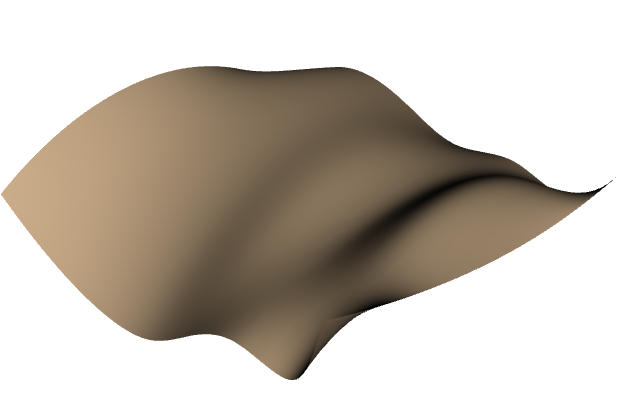
\includegraphics[width=1.0\textwidth]{figures/basic_usage_trans.png}
            \end{column}
        \end{columns}
    \end{center}

\end{frame}

%%%%%%%%%%%%%%%%%%%%%%%%%%%%%%%%%%%%%%%%%%%%%%%%%%%%%%%%%%%%%%%%%%%%%%%%%%%%%%%
\subsection{Basic Volumetric Plotting}
\begin{frame}
    \frametitle{Examples - Basic Volumetric Plot}

    Load a volumetric dataset from the built-in examples and plot it.

    \begin{center}
        \begin{columns}[T]
            \begin{column}{.5\textwidth}
                \inputminted[fontsize=\footnotesize]{python}{code/basic_usage2.py}
            \end{column}

            \begin{column}{.5\textwidth}
                \centering
                \vspace{5pt}
                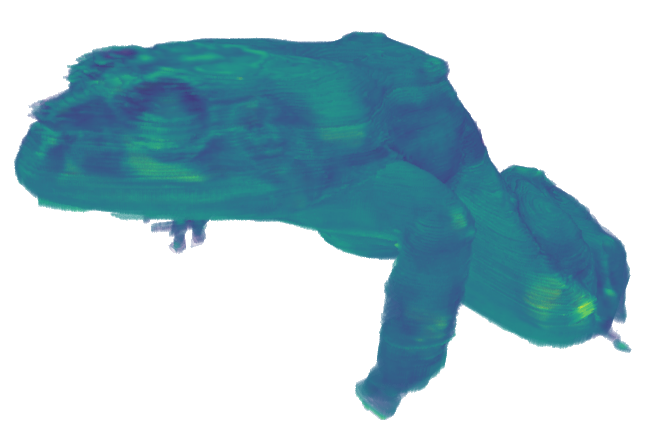
\includegraphics[width=1.0\textwidth]{figures/basic_usage2_trans.png}
            \end{column}
        \end{columns}
    \end{center}

\end{frame}

%%%%%%%%%%%%%%%%%%%%%%%%%%%%%%%%%%%%%%%%%%%%%%%%%%%%%%%%%%%%%%%%%%%%%%%%%%%%%%%
\subsection{Filters}
\begin{frame}
    \frametitle{Examples - Filters}

    \begin{center}
        \begin{columns}[T]
            \begin{column}{.5\textwidth}
                \inputminted[fontsize=\footnotesize]{python}{code/filters.py}
            \end{column}

            \begin{column}{.5\textwidth}
                \centering
                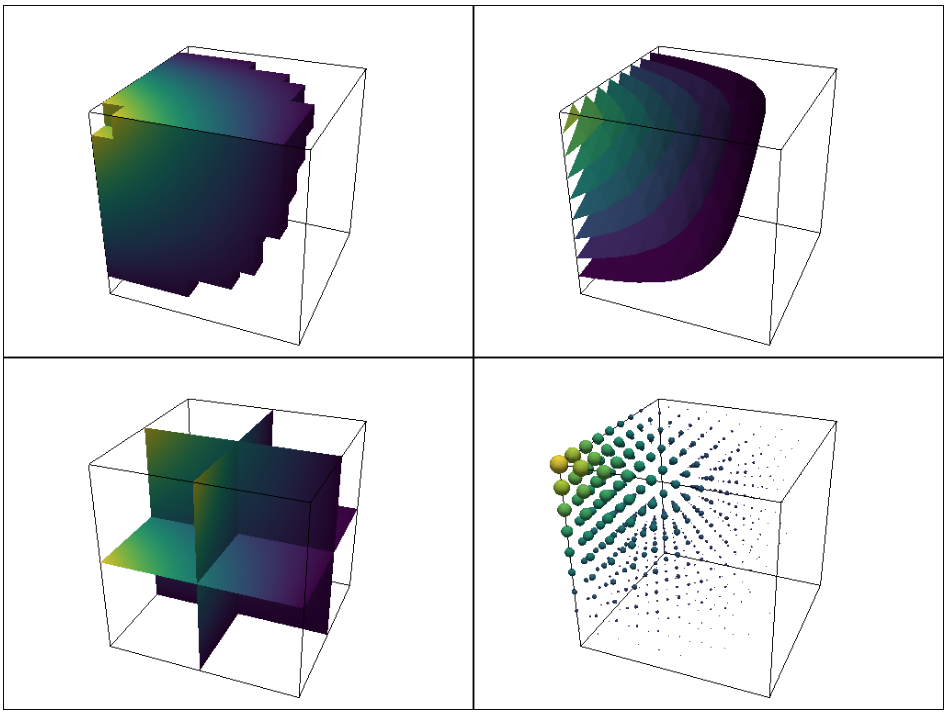
\includegraphics[width=1.0\textwidth]{figures/filters_trans.png}
            \end{column}
        \end{columns}
    \end{center}

\end{frame}

%%%%%%%%%%%%%%%%%%%%%%%%%%%%%%%%%%%%%%%%%%%%%%%%%%%%%%%%%%%%%%%%%%%%%%%%%%%%%%%
\begin{frame}
    \frametitle{Examples - Widgets}

    Demonstrate interactive filters by loading a mesh and modifying the resolution of a VTK pipeline.

    \begin{center}
        \begin{columns}[T]
            \begin{column}{.4\textwidth}
                \inputminted[fontsize=\footnotesize]{python}{code/widgets_ex.py}
            \end{column}

            \begin{column}{.6\textwidth}
                \centering
                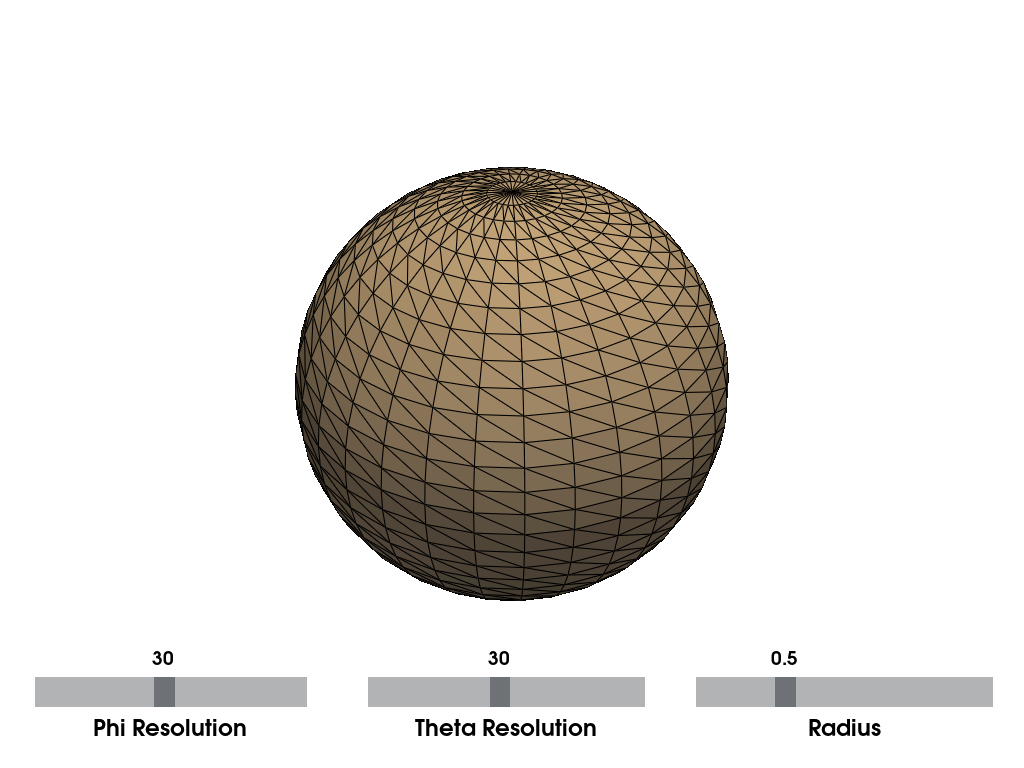
\includegraphics[width=1.0\textwidth]{figures/sphx_glr_d_multi-slider-widget_001_trans.png}
            \end{column}
        \end{columns}
    \end{center}

\end{frame}

%%%%%%%%%%%%%%%%%%%%%%%%%%%%%%%%%%%%%%%%%%%%%%%%%%%%%%%%%%%%%%%%%%%%%%%%%%%%%%%
\section{Extending PyVista: Deployment, Packaging, and Documentation}

%%%%%%%%%%%%%%%%%%%%%%%%%%%%%%%%%%%%%%%%%%%%%%%%%%%%%%%%%%%%%%%%%%%%%%%%%%%%%%%

\subsection{PyInstaller and PyQT}
\begin{frame}
\frametitle{Examples - PyInstaller and PyQT}

\begin{center}
    \begin{columns}[T]
        \begin{column}{.5\textwidth}
            \small
            \begin{itemize}[leftmargin=8pt, label=•]
                \item Use PyInstaller and PyQT or PySide to create a standalone application.
                \item Multi-platform. Build on the OS you intend to deploy.
                \item Compatible with GitHub Actions and can be automated.
                \item Deploy as using an installer like NSIS.
            \end{itemize}
            \vspace{15pt}
        \end{column}

        \begin{column}{.5\textwidth}
            \centering
            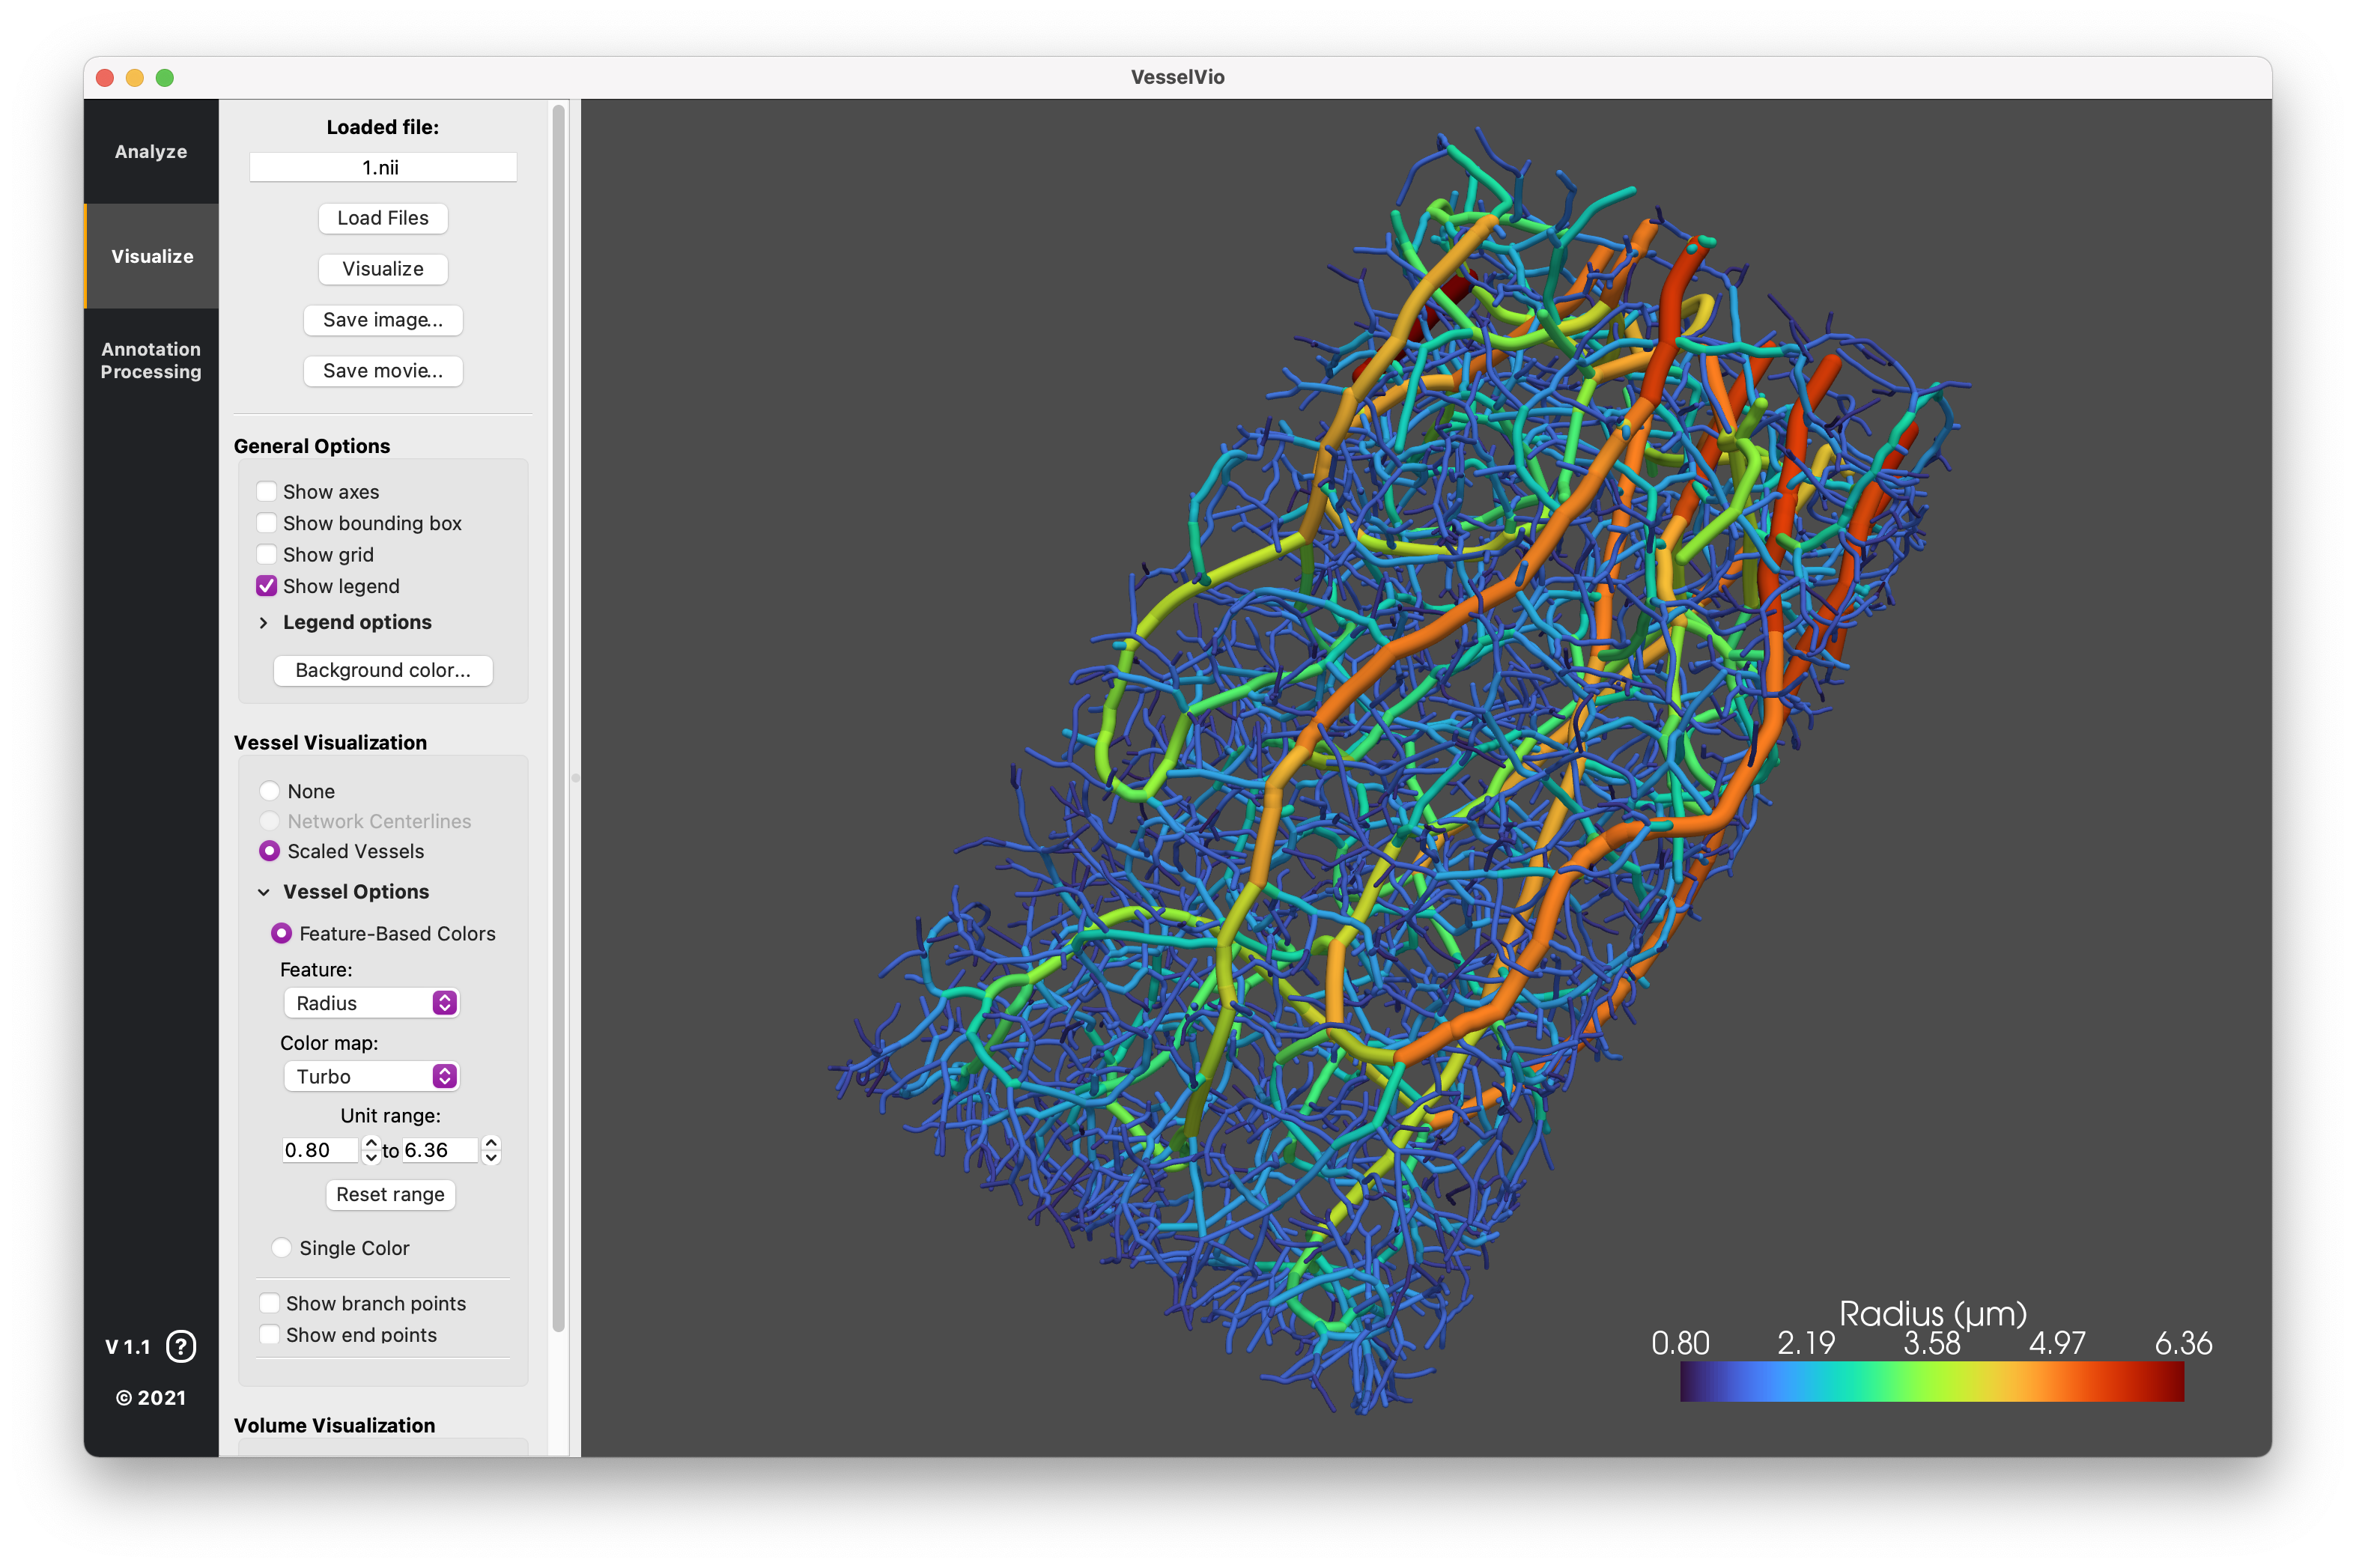
\includegraphics[width=1.0\textwidth]{figures/VesselVio.png}
        \end{column}
    \end{columns}

\end{center}

\begin{center}
\inputminted[fontsize=\footnotesize]{bash}{code/pyinstaller.py}
\end{cernter}

\end{frame}

%%%%%%%%%%%%%%%%%%%%%%%%%%%%%%%%%%%%%%%%%%%%%%%%%%%%%%%%%%%%%%%%%%%%%%%%%%%%%%%
\begin{frame}
    \frametitle{Examples - Documentation with Sphinx}

    \begin{center}
        \begin{columns}[T]
            \begin{column}{.5\textwidth}
                \small
                \begin{itemize}[leftmargin=10pt, label=•]
                    \item PyVista supports the Sphinx documentation generator.
                    \item Allows you to generate static and interactive documentation.
                    \item Place code snippets directly in the documentation as examples.
                \end{itemize}
                \vspace{40pt}
                \inputminted[fontsize=\footnotesize]{bash}{code/sphinx_conf.py}
            \end{column}

            \begin{column}{.5\textwidth}
                \vspace{-5pt}
                \centering
                \href{https://docs.pyvista.org/}{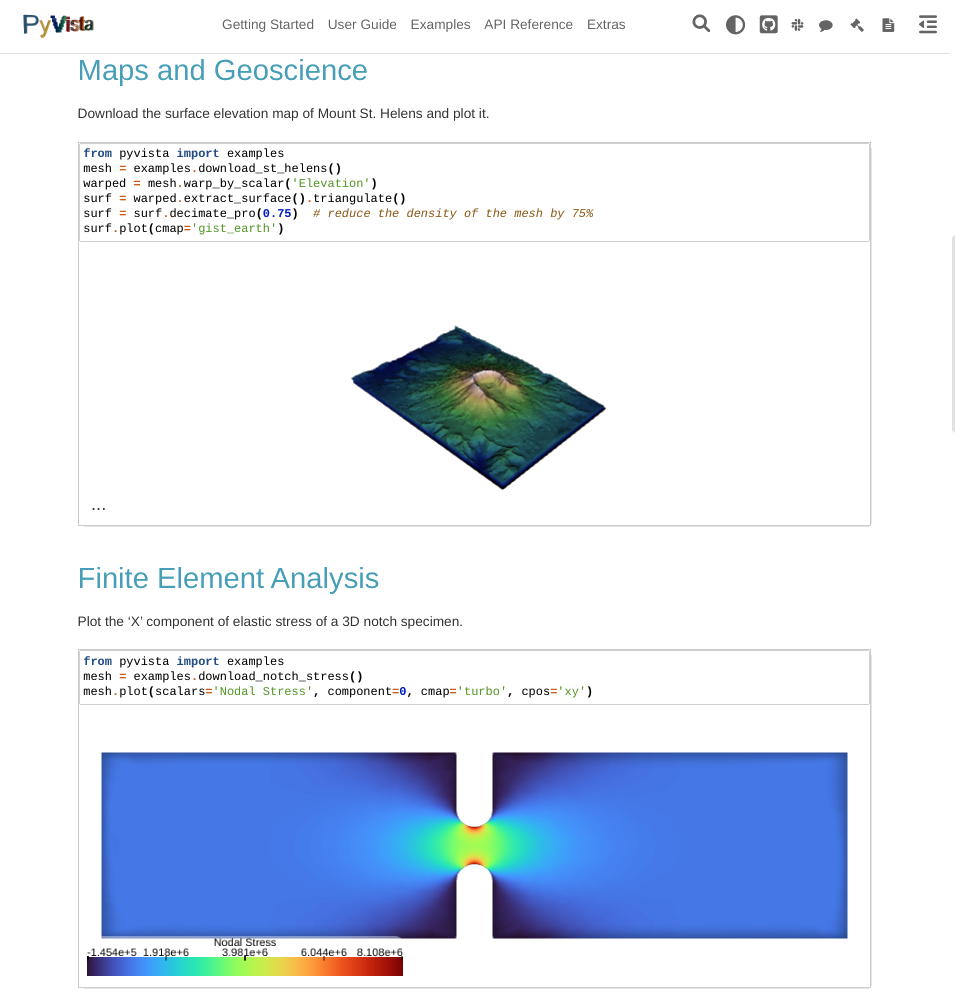
\includegraphics[width=0.9\textwidth]{figures/sphinx-trans.png}}
            \end{column}
        \end{columns}
    \end{center}

\end{frame}

%%%%%%%%%%%%%%%%%%%%%%%%%%%%%%%%%%%%%%%%%%%%%%%%%%%%%%%%%%%%%%%%%%%%%%%%%%%%%%%
\section{PyVista - Ecosystem}

\begin{frame}

    \frametitle{PyVista - Ecosystem}
    
\includegraphics[width=1.0\textwidth]{figures/pyvista-repo.png}

    \begin{itemize}[leftmargin=10pt, label=•]
        \item \textbf{\href{https://github.com/pyvista/pymeshfix}{pymeshfix}} - Python Wrapper for MeshFix: Easily repair holes in surface meshes
        \item \textbf{\href{https://github.com/pyvista/tetgen}{tetgen}} - Generate tetrahedral meshes of any 3D polyhedral domain
        \item \textbf{\href{https://github.com/pyvista/PyACVD}{PyACVD}} - Python implementation of surface mesh resampling algorithm ACVD
        \item \textbf{\href{https://github.com/pyvista/fast-simplification}{fast-simplification}} - Fast Quadratic Mesh Simplification
        \item \textbf{\href{https://github.com/pyvista/pyvista-qt}{pyvista-qt}} - Qt support for PyVista
        \item \textbf{\href{https://github.com/pyvista/pyvista-xarray}{pyvista-xarray}} - xarray DataArray accessors for PyVista
    \end{itemize}

\end{frame}

%%%%%%%%%%%%%%%%%%%%%%%%%%%%%%%%%%%%%%%%%%%%%%%%%%%%%%%%%%%%%%%%%%%%%%%%%%%%%%%
\subsection{Tutorial}
\begin{frame}
    \frametitle{Tutorial}

    The \href{https://tutorial.pyvista.org}{PyVista Tutorial} contains a variety of lessons to help you get started with PyVista. Includes:

    \begin{itemize}[leftmargin=10pt, label=•]
        \item Introduction - Using PyVista for 3D Visualization within Python.
        \item Reading and plotting 3D data using the PyVista module and external files.
        \item Learn the basics of the PyVista data types and how to open common 3D file formats to visualize the data in 3D.
        \item Demonstrate many features of the PyVista plotting API to create compelling 3D visualizations and touch on animations.
        \item Demonstrate the PyVista filters API to perform mesh analysis and alteration.
    \end{itemize}

\end{frame}

%%%%%%%%%%%%%%%%%%%%%%%%%%%%%%%%%%%%%%%%%%%%%%%%%%%%%%%%%%%%%%%%%%%%%%%%%%%%%%%
\section{PyVista Applied to CAE Datasets}

\subsection{Introduction}
\begin{frame}

    \frametitle{PyVista Applied to CAE Datasets - Introduction}

    \begin{itemize}[leftmargin=10pt, label=•]
        \item \textbf{Built on the Best:} Built on VTK, PyVista simplifies complex CAE data processing while maintaining full compatibility with industry-standard formats.
        \item \textbf{Efficient Data Handling:} Supports large-scale meshes, point clouds, volumetric data, and time-dependent simulations with optimized memory management.
        \item \textbf{Advanced Visualization:} Enables rapid 3D rendering of simulation results, including contouring, slicing, and isosurfacing.
        \item \textbf{Interactivity:} Provides interactive plotting tools and GUI integration for intuitive CAE analysis.
        \item \textbf{Extensive Filtering & Processing:} Leverages powerful mesh manipulation and computational tools, ideal for FEA, CFD, and structural simulations.
        \item \textbf{Automation & Scripting:} Python-based, making it easy to integrate with CAE workflows for automated post-processing and analysis.
    \end{itemize}

\end{frame}

%%%%%%%%%%%%%%%%%%%%%%%%%%%%%%%%%%%%%%%%%%%%%%%%%%%%%%%%%%%%%%%%%%%%%%%%%%%%%%%
\begin{frame}
    \frametitle{PyVista - CAE Usage}

    PyVista is widely used to alongside structural and CFD simulations,
    offering efficient visualization and analysis of simulation results. Its
    integration with VTK enables handling large datasets, automating workflows,
    and enhancing data interpretation.

    \begin{columns}[T]
        \begin{column}{.3\textwidth}
            \begin{customexampleblock}{\small Structural - Static Results}
                \centering
                \begin{minipage}[c][3cm][c]{\textwidth}
                    \href{https://www.simscale.com/dashboard/projects/794804934725811465}{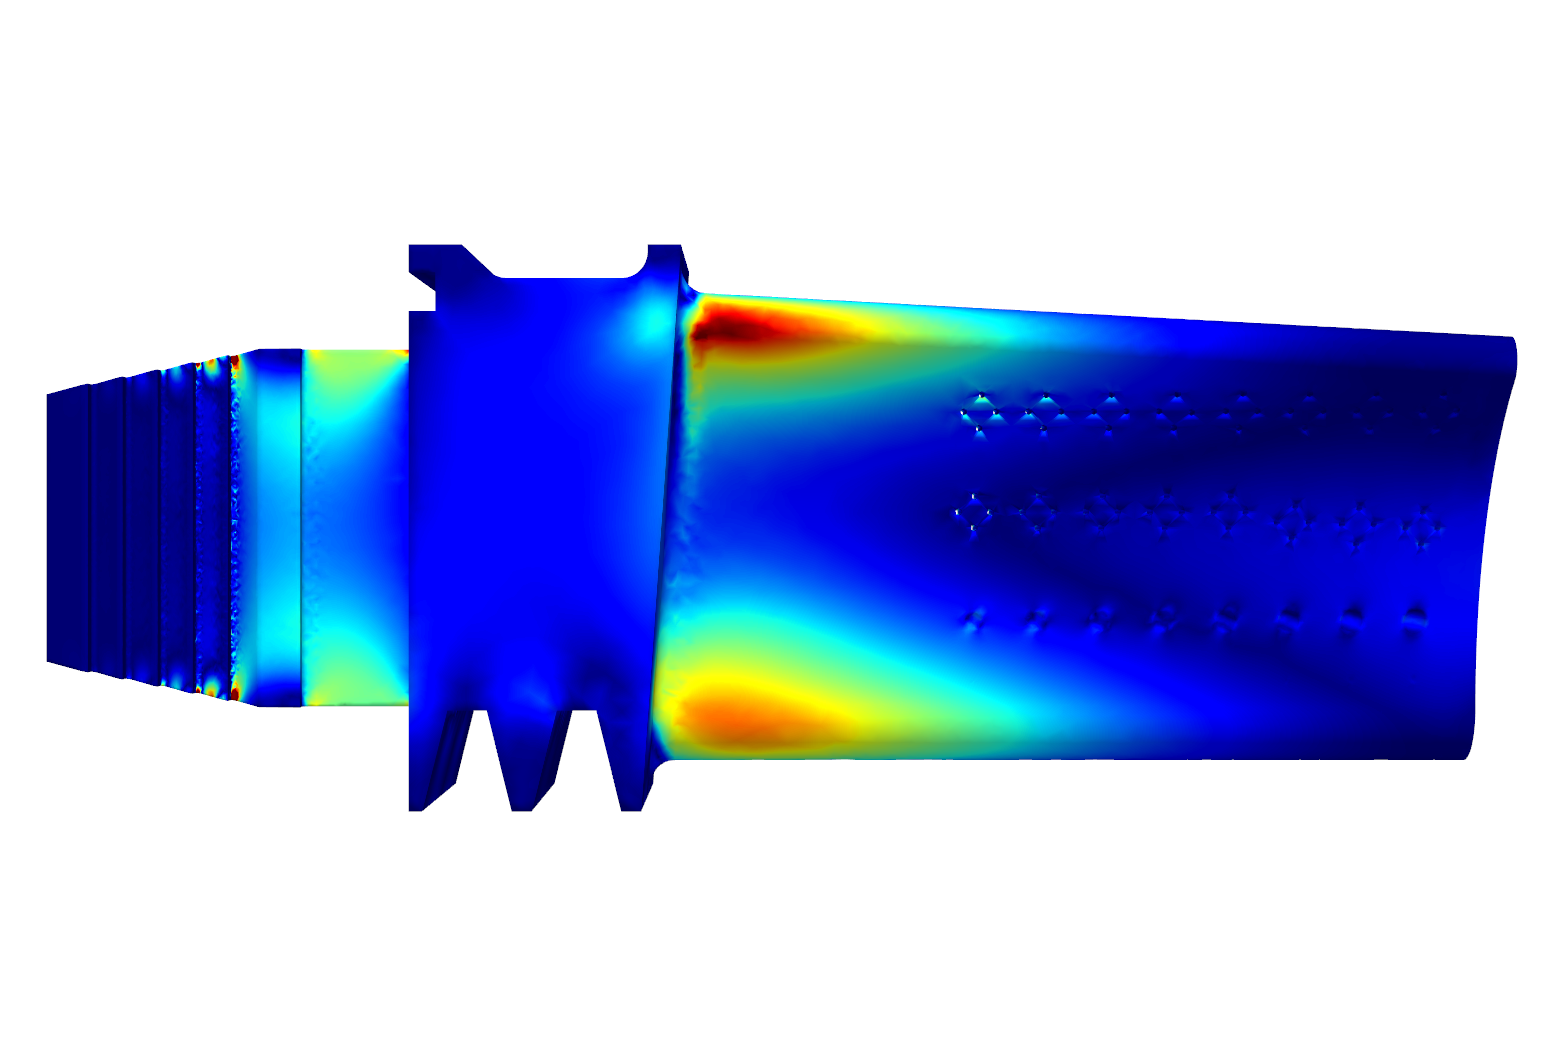
\includegraphics[width=\textwidth,height=3.5cm,keepaspectratio]{figures/turbine-static-trans.png}}
                \end{minipage}
            \end{customexampleblock}
        \end{column}

        \begin{column}{.3\textwidth}
            \begin{customexampleblock}{\small Structural - Modal Analysis}
                \centering
                \begin{minipage}[c][3cm][c]{\textwidth}
                    \href{https://asmedigitalcollection.asme.org/GT/proceedings-abstract/GT2020/84232/V011T30A029/1095393?redirectedFrom=PDF}{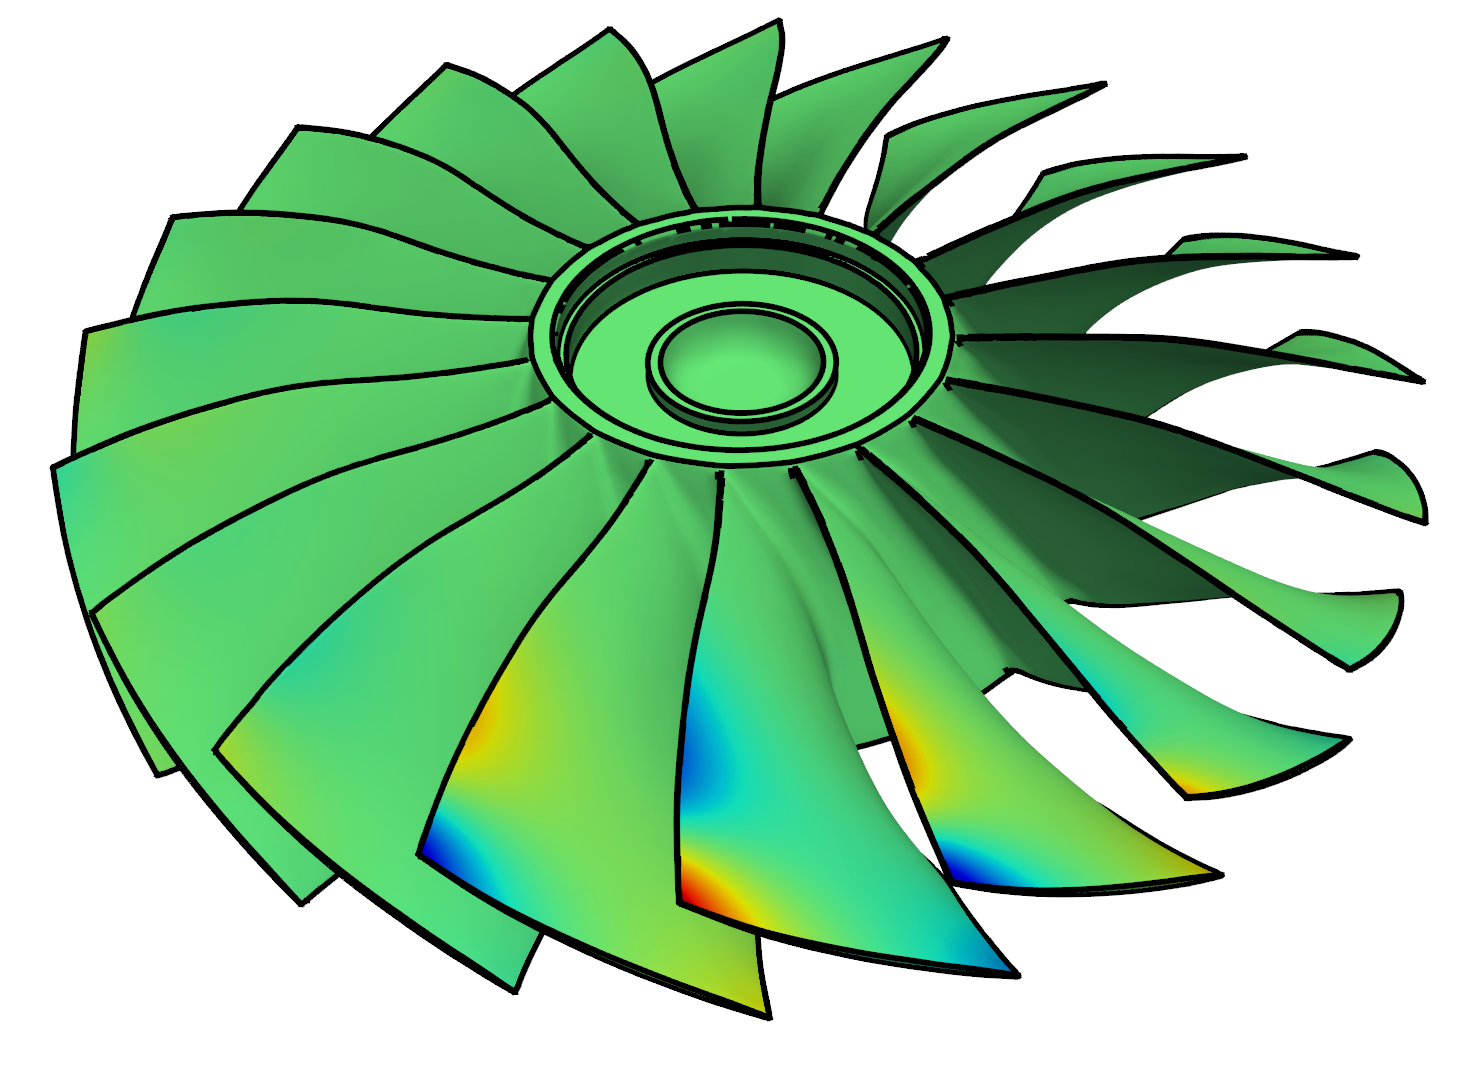
\includegraphics[width=\textwidth,height=3.5cm,keepaspectratio]{figures/PBS-mode-94-trans.png}}
                \end{minipage}
            \end{customexampleblock}
        \end{column}

        \begin{column}{.3\textwidth}
            \begin{customexampleblock}{\small CFD - Steady and Turbulent}
                \centering
                \begin{minipage}[c][3cm][c]{\textwidth}
                    \href{https://pasteurlabs.ai/}{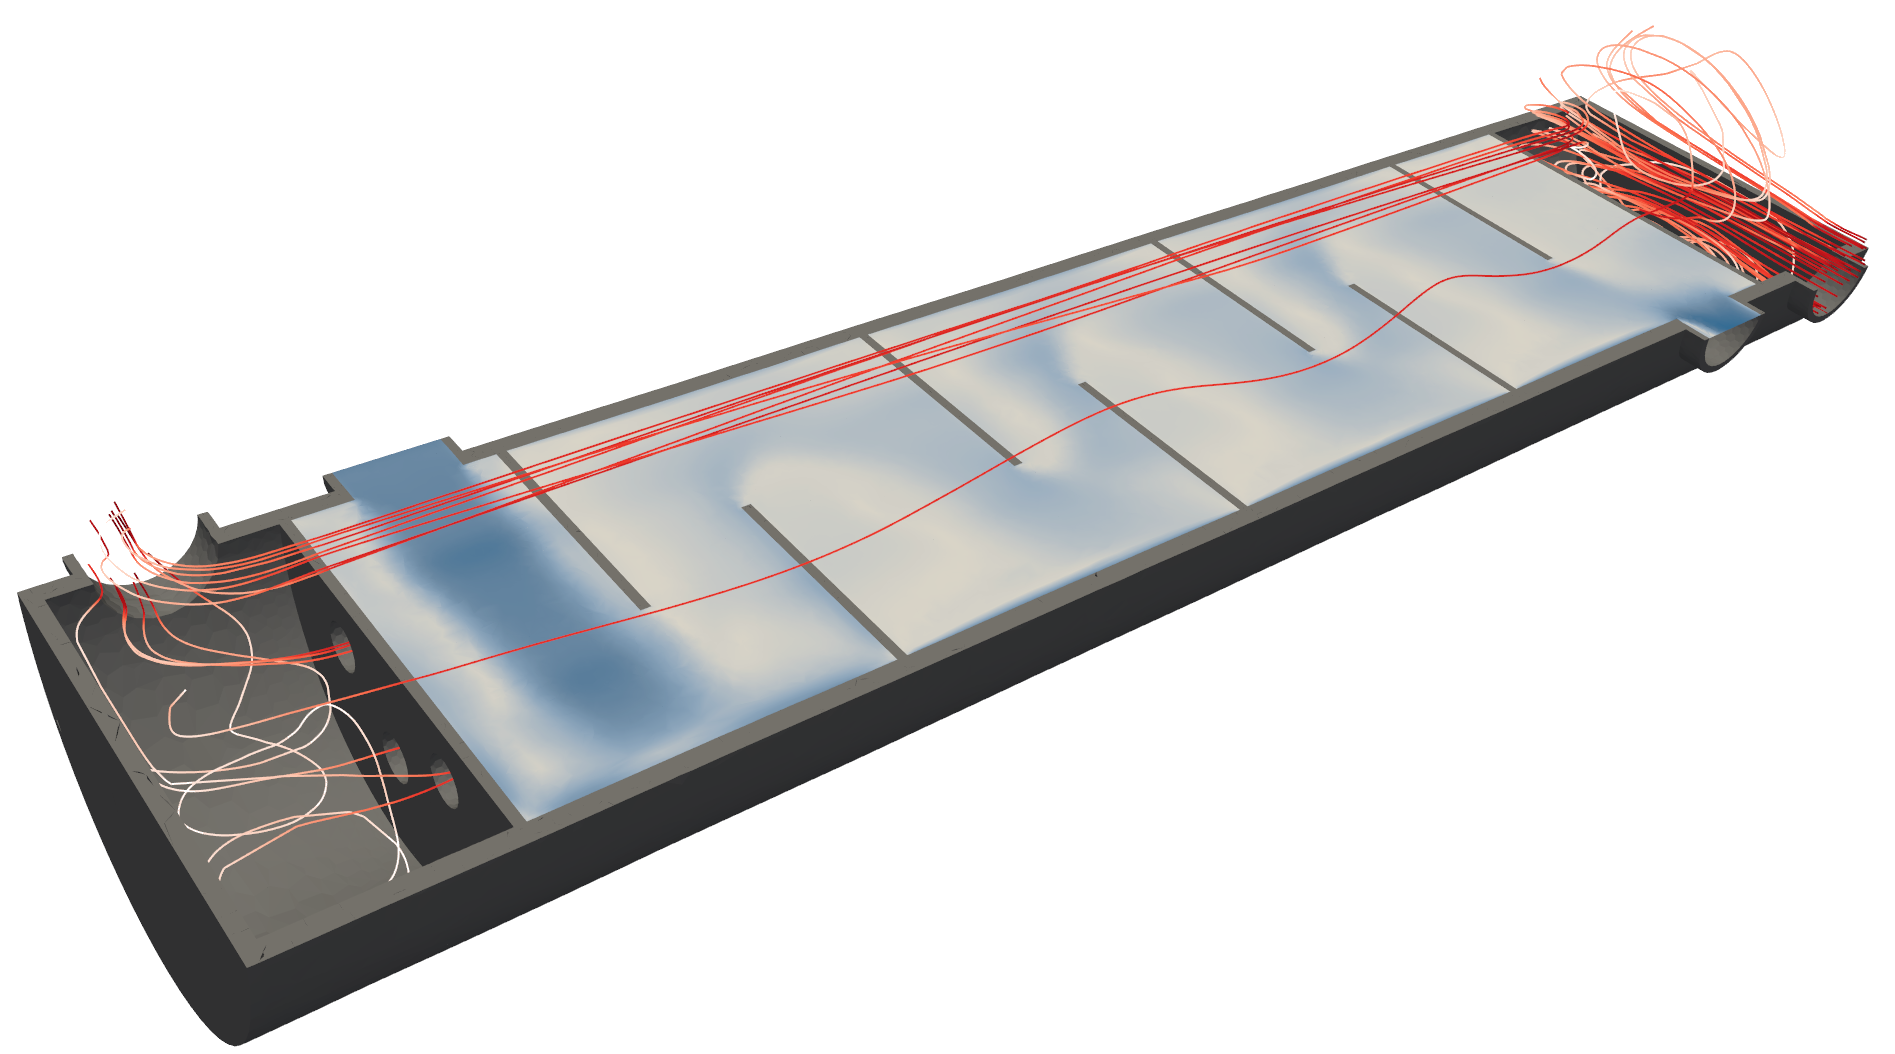
\includegraphics[width=\textwidth,height=3.5cm,keepaspectratio]{figures/heat-exchanger-trans.png}}
                \end{minipage}
            \end{customexampleblock}
        \end{column}
    \end{columns}

\end{frame}

%%%%%%%%%%%%%%%%%%%%%%%%%%%%%%%%%%%%%%%%%%%%%%%%%%%%%%%%%%%%%%%%%%%%%%%%%%%%%%%
\subsection{Jupyterlab Demos}

%%%%%%%%%%%%%%%%%%%%%%%%%%%%%%%%%%%%%%%%%%%%%%%%%%%%%%%%%%%%%%%%%%%%%%%%%%%%%%%
\begin{frame}

    \frametitle{Jupyterlab Demos}

    \begin{center}
        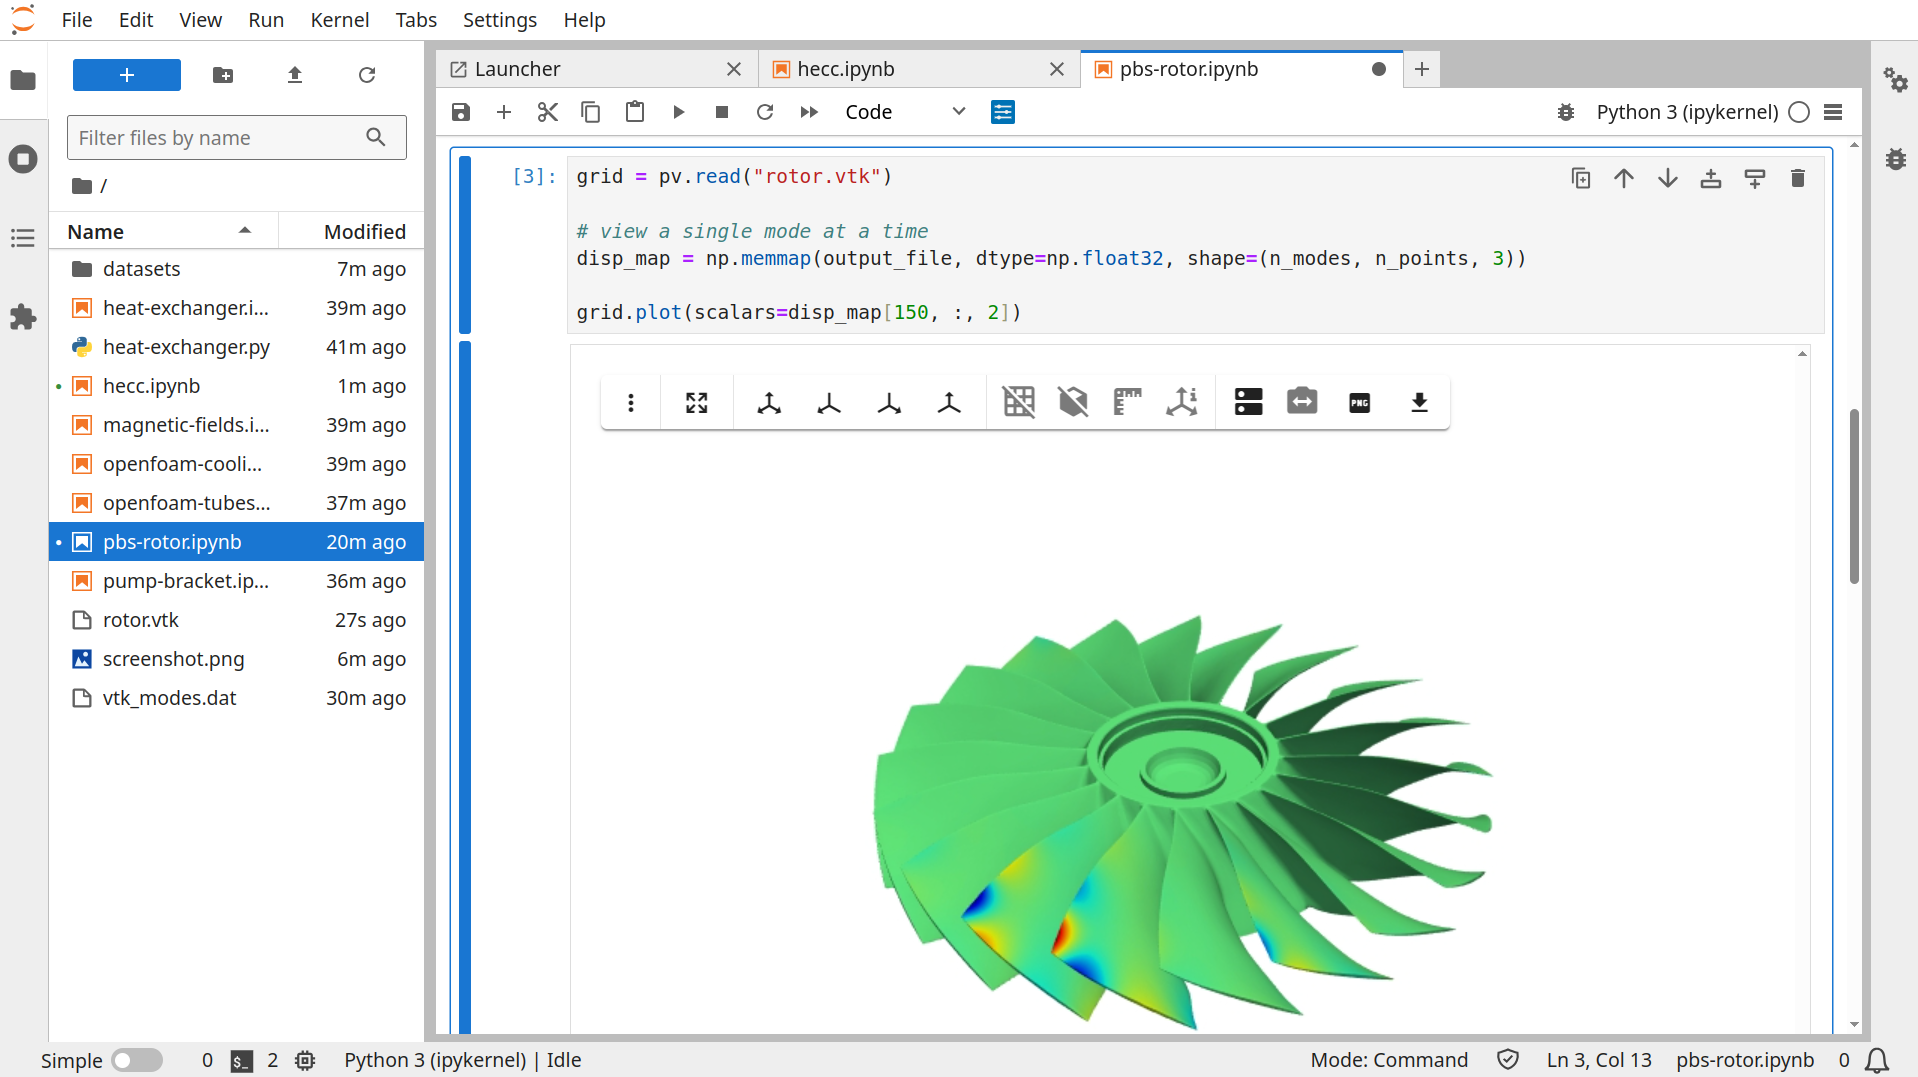
\includegraphics[width=1.0\textwidth]{figures/jupyterlab.png}
    \end{center}

\end{frame}

%%%%%%%%%%%%%%%%%%%%%%%%%%%%%%%%%%%%%%%%%%%%%%%%%%%%%%%%%%%%%%%%%%%%%%%%%%%%%%%
\subsection{Surface Scan Analysis - HECC}
\begin{frame}

    \frametitle{Surface Scan Analysis - HECC}

    \href{https://ntrs.nasa.gov/citations/20180001471}{High Efficiency Centrifugal Compressor for Rotorcraft Applications}

    Plotting and demonstrating filters on the 4.5M point surface scan.

    \begin{center}

        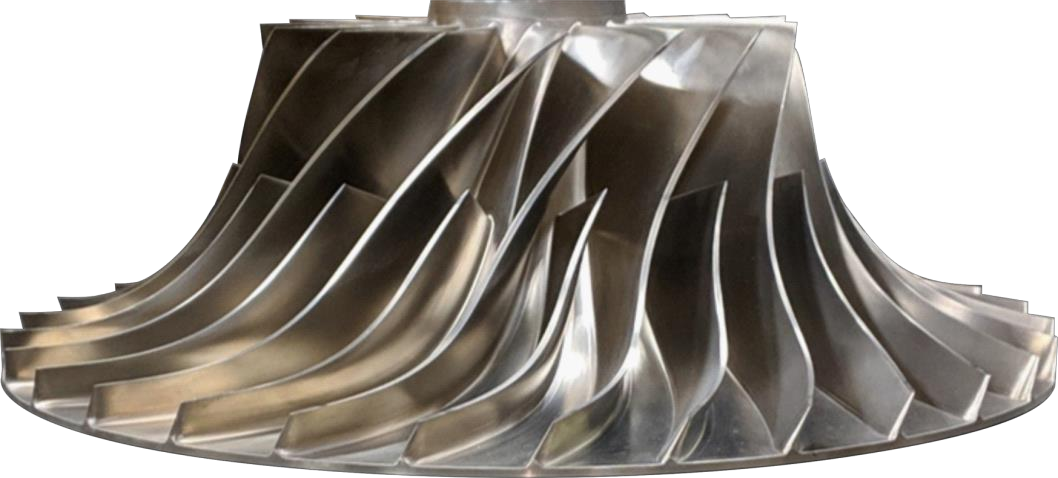
\includegraphics[width=1.0\textwidth]{figures/hecc-rotor-real.png}

    \end{center}

\end{frame}

%%%%%%%%%%%%%%%%%%%%%%%%%%%%%%%%%%%%%%%%%%%%%%%%%%%%%%%%%%%%%%%%%%%%%%%%%%%%%%%
\begin{frame}

    \frametitle{Surface Scan Analysis - HECC}

    \inputminted[fontsize=\footnotesize]{python}{code/hecc-1.py}

\end{frame}

%%%%%%%%%%%%%%%%%%%%%%%%%%%%%%%%%%%%%%%%%%%%%%%%%%%%%%%%%%%%%%%%%%%%%%%%%%%%%%%
\begin{frame}

    \frametitle{Surface Scan Analysis - HECC}

    \begin{center}

        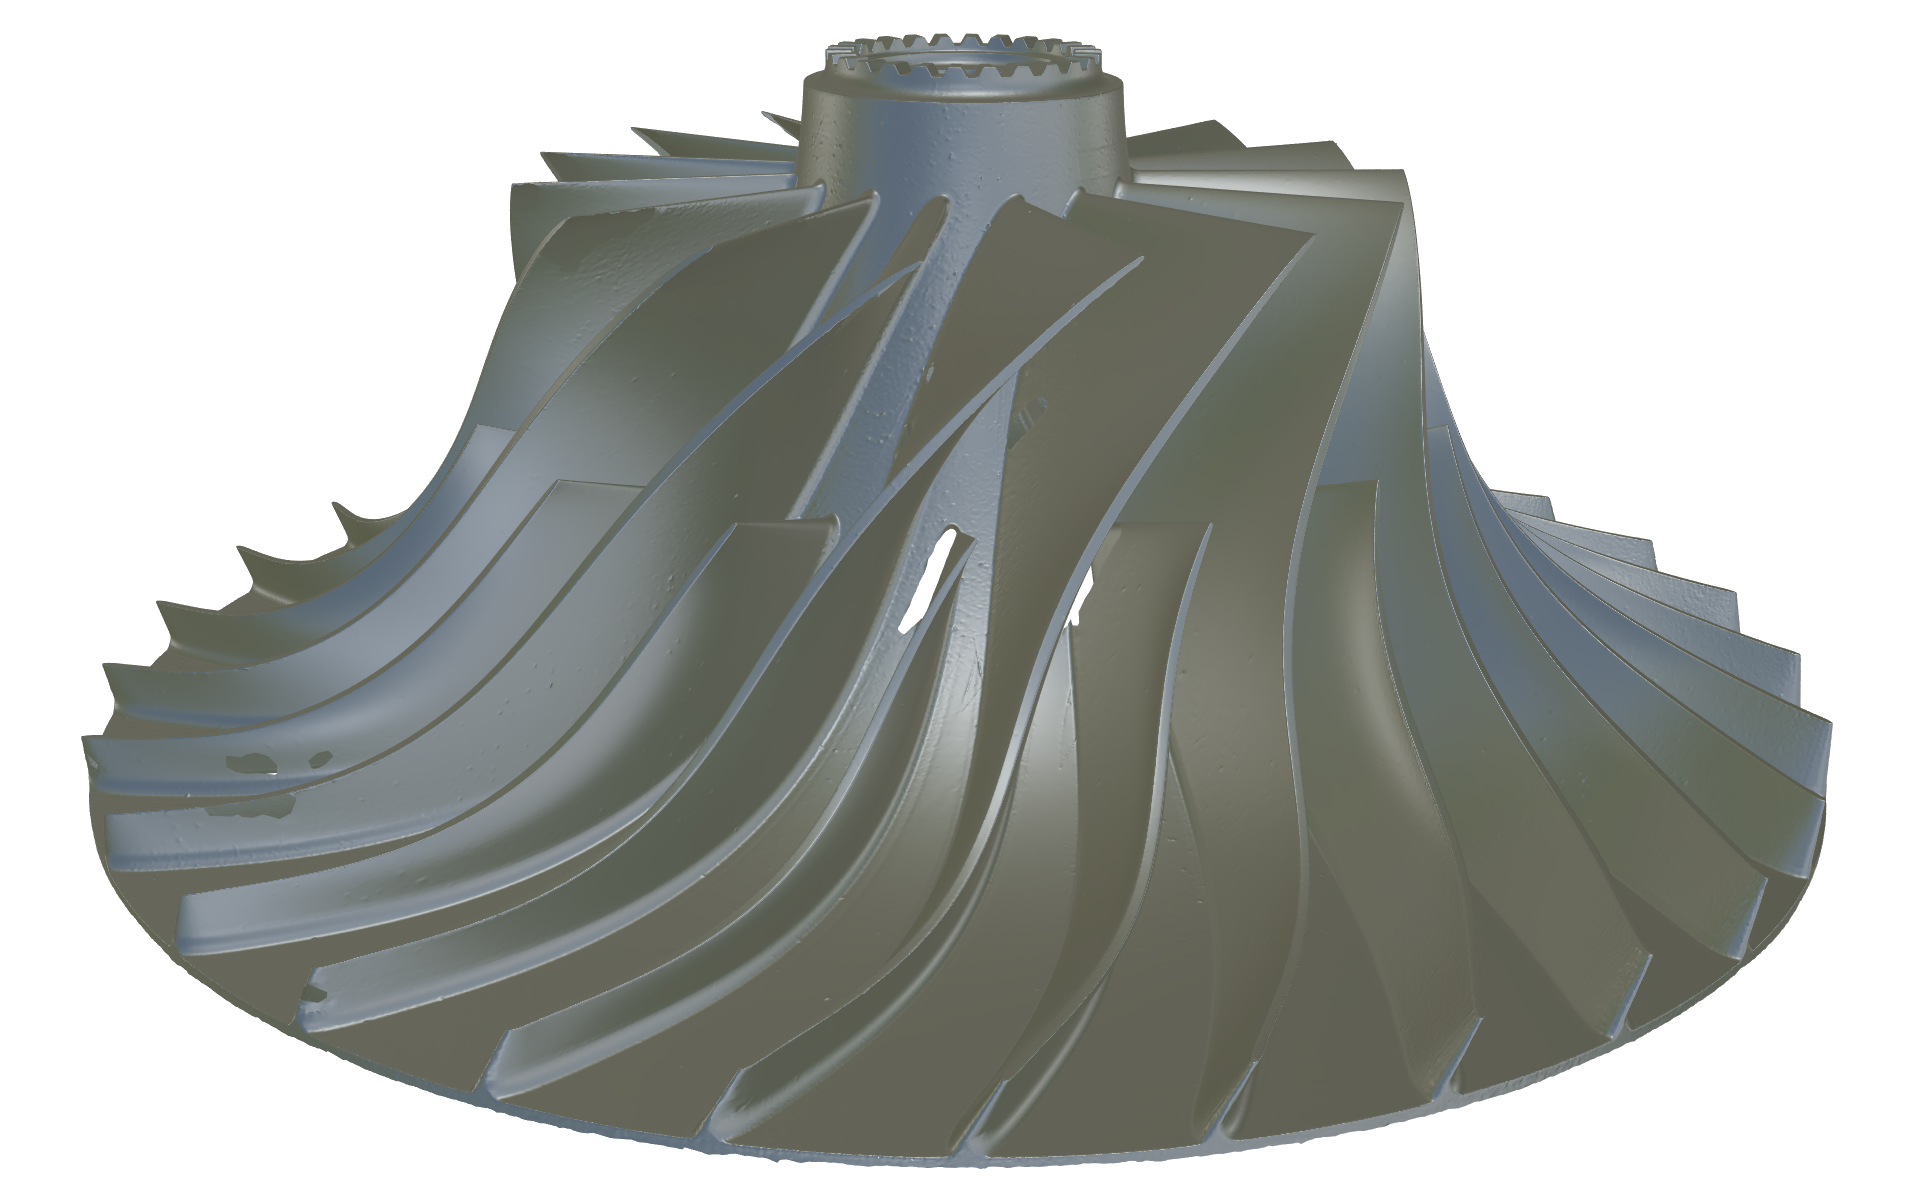
\includegraphics[width=1.0\textwidth]{figures/hecc-rotor-pbr-trans.png}

    \end{center}

\end{frame}

%%%%%%%%%%%%%%%%%%%%%%%%%%%%%%%%%%%%%%%%%%%%%%%%%%%%%%%%%%%%%%%%%%%%%%%%%%%%%%%
\begin{frame}

    \frametitle{Surface Scan Analysis - HECC}
    \inputminted[fontsize=\footnotesize]{python}{code/hecc-2.py}

\end{frame}

%%%%%%%%%%%%%%%%%%%%%%%%%%%%%%%%%%%%%%%%%%%%%%%%%%%%%%%%%%%%%%%%%%%%%%%%%%%%%%%
\begin{frame}

    \frametitle{Surface Scan Analysis - HECC}

    \begin{center}
        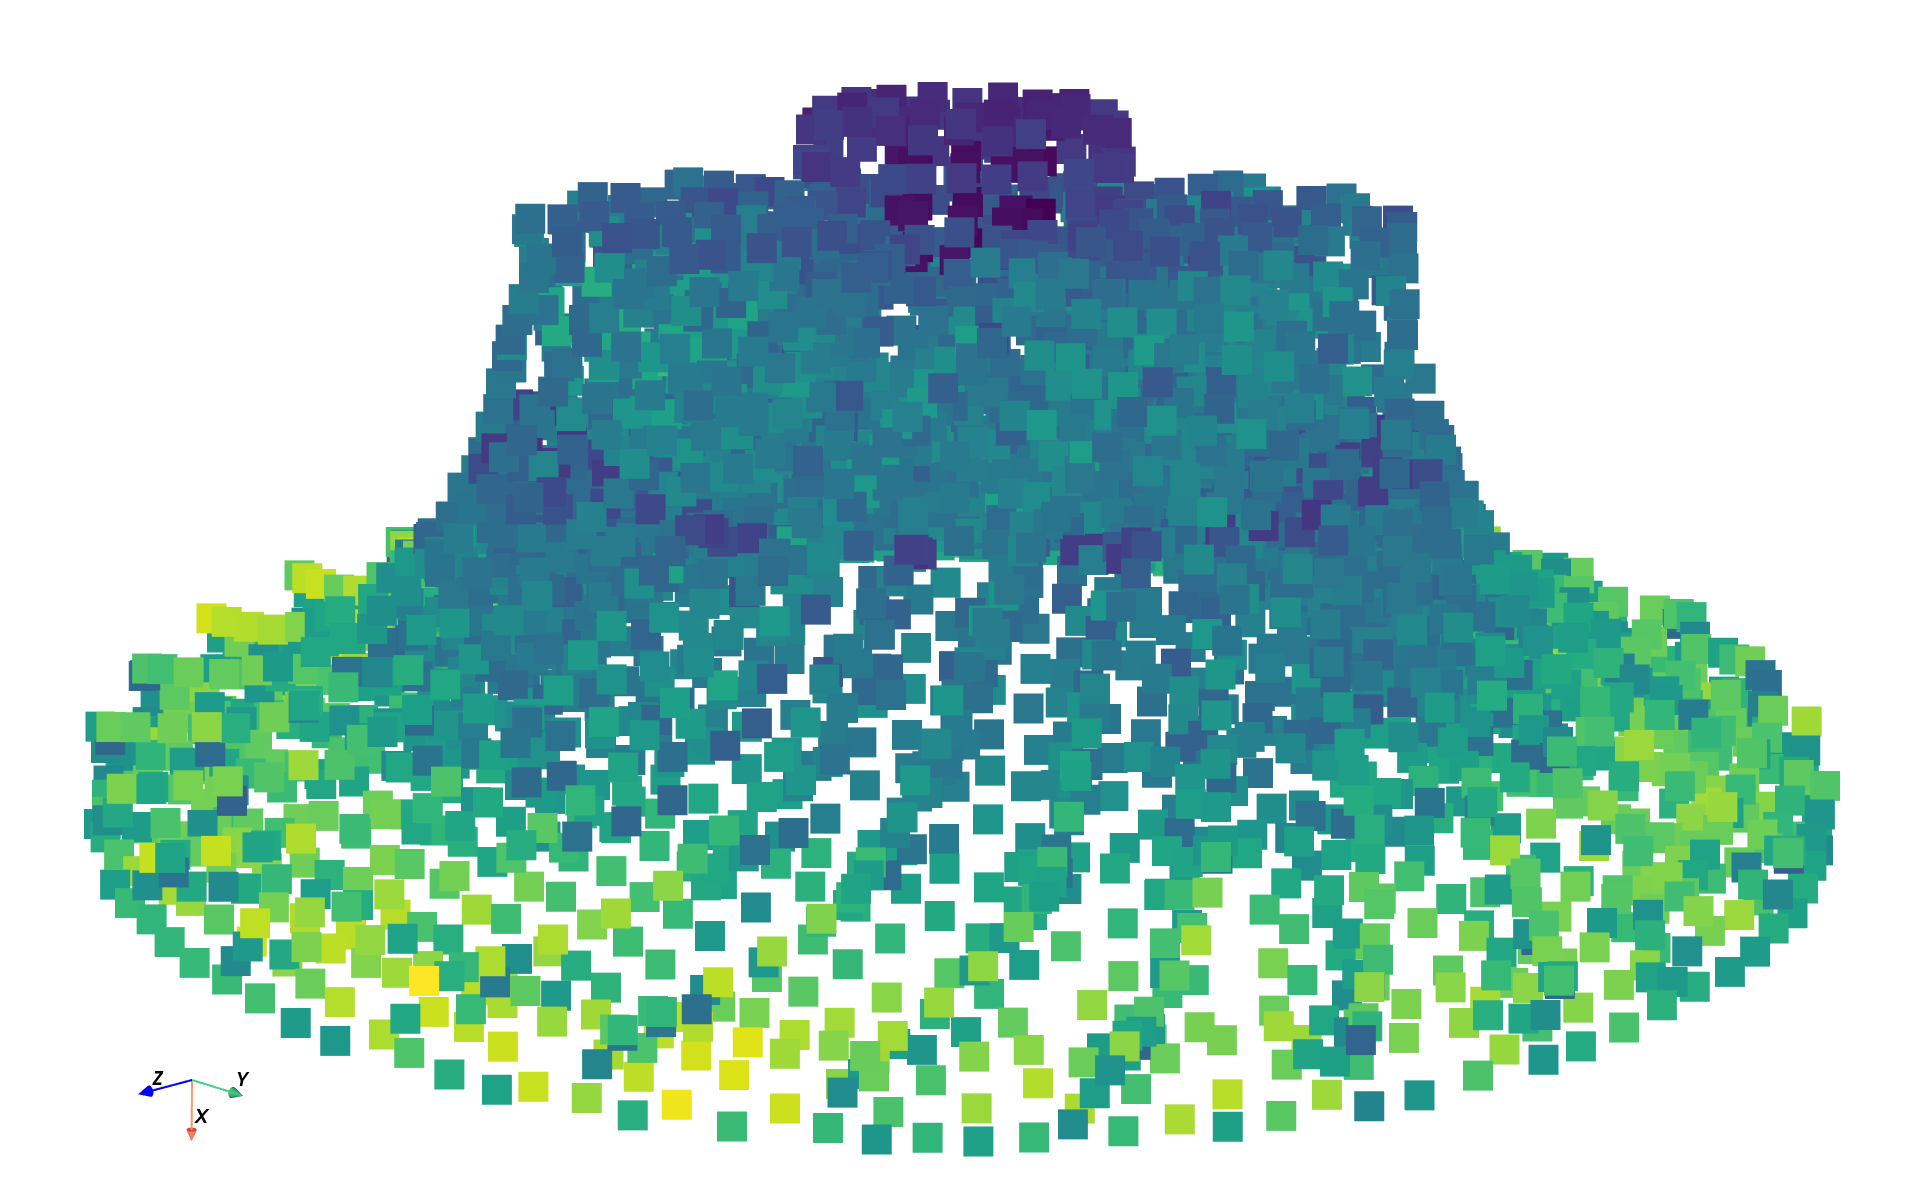
\includegraphics[width=1.0\textwidth]{figures/hecc-rotor-pfh-pointset.png}
    \end{center}

\end{frame}

%%%%%%%%%%%%%%%%%%%%%%%%%%%%%%%%%%%%%%%%%%%%%%%%%%%%%%%%%%%%%%%%%%%%%%%%%%%%%%%
\begin{frame}

    \frametitle{Single Page Applications using Panel}

    \begin{center}
        \href{https://panel-example-production.up.railway.app/}{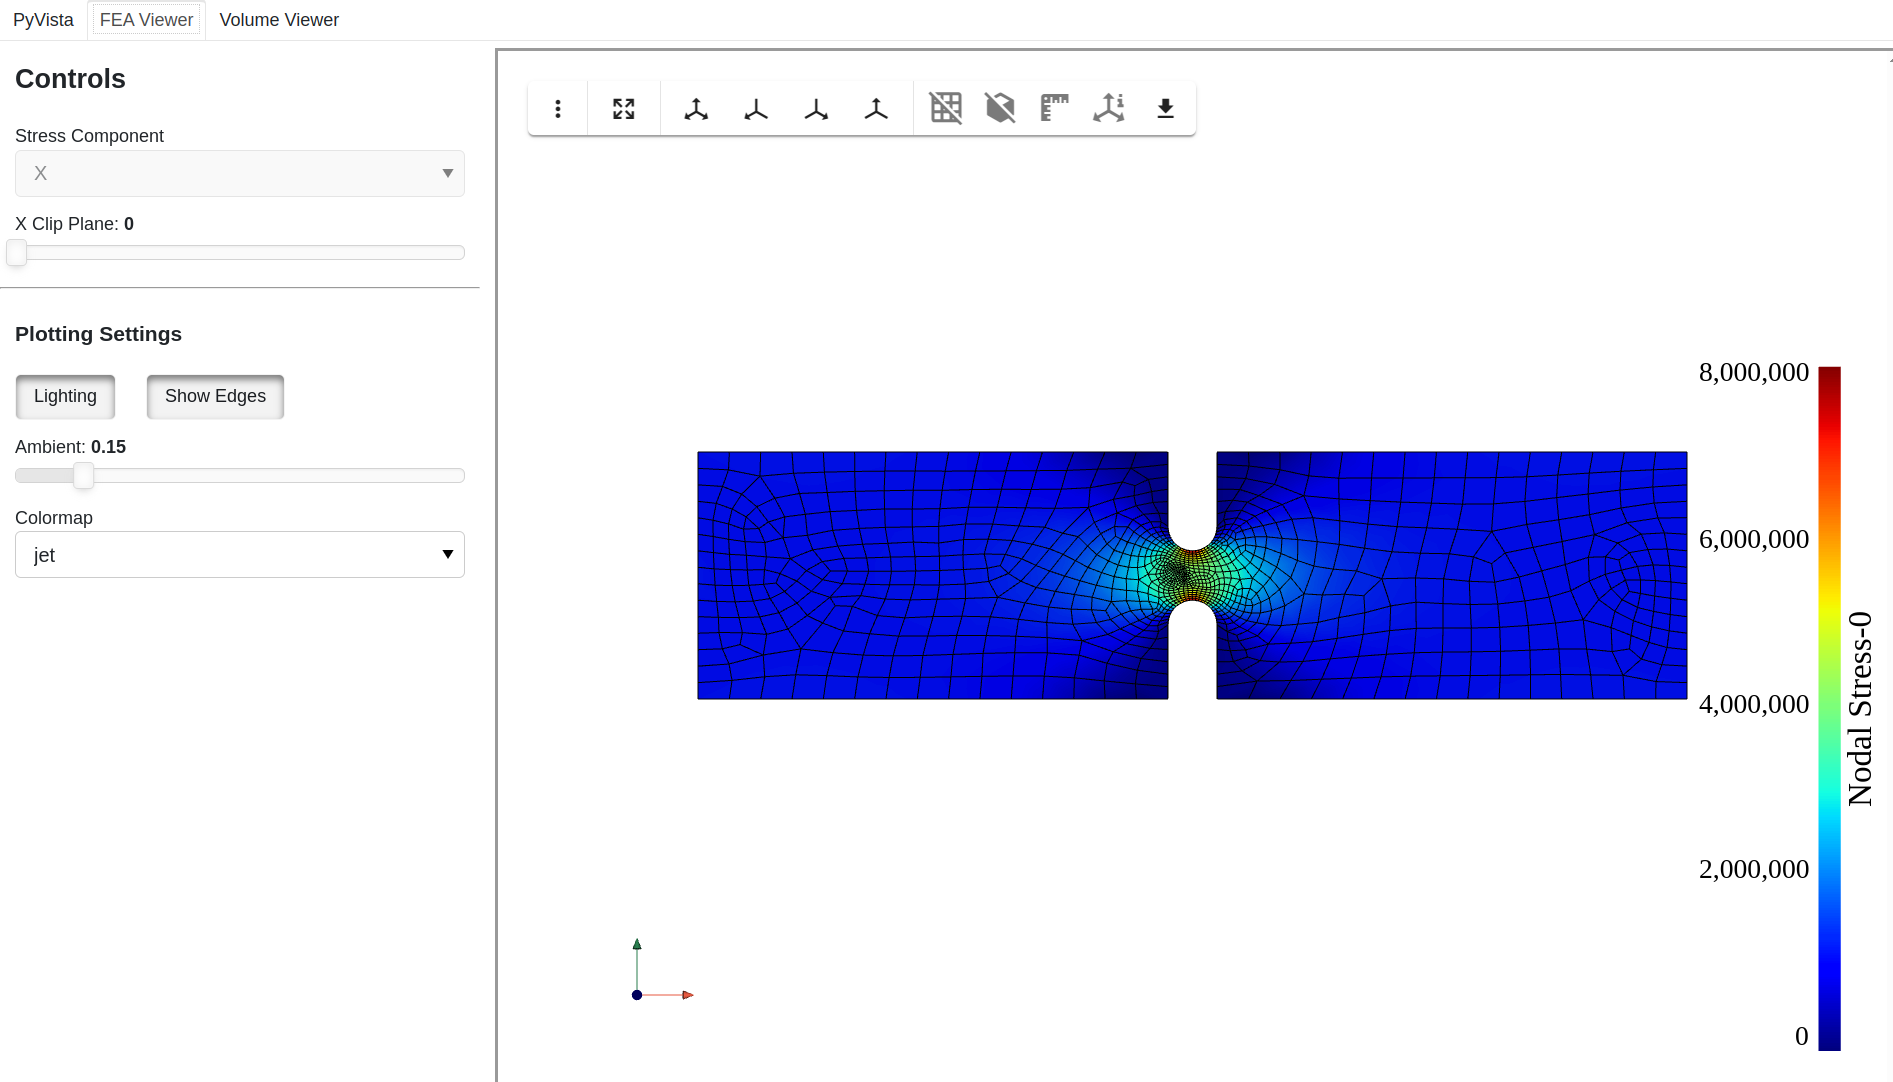
\includegraphics[width=\textwidth]{figures/panel-pyvista.png}}
    \end{center}

\end{frame}

%%%%%%%%%%%%%%%%%%%%%%%%%%%%%%%%%%%%%%%%%%%%%%%%%%%%%%%%%%%%%%%%%%%%%%%%%%%%%%%
\begin{frame}
    \frametitle{Further Resources and Support}

    \centering
    \textbf{Tutorial:} \\[5pt]
    \href{https://tutorial.pyvista.org/}{tutorial.pyvista.org} \\[10pt]

    \textbf{Community Discussions (General Usage):} \\[5pt]
    \href{https://github.com/pyvista/pyvista/discussions}{github.com/pyvista/pyvista/discussions} \\[10pt]

    \textbf{Issue Tracking and Feature Requests:} \\[5pt]
    \href{https://github.com/pyvista/pyvista/issues}{github.com/pyvista/pyvista/issues} \\[10pt]

    \textbf{Professional Support:} \\[5pt]
    \href{https://www.kitware.com/support/}{Kitware Support Services} \\[10pt]

    \rule{\textwidth}{0.5pt}

    \textbf{Contact:} \\[5pt]
    GitHub: \href{https://github.com/akaszynski}{@akaszynski} \\[5pt]
    %% Email: \href{mailto:akascap@gmail.com}{akascap@gmail.com} \\[10pt]
    Email: \href{mailto:Alex.Kaszynski@simulation.science}{Alex.Kaszynski@simulation.science} \\[10pt]

\end{frame}

%%%%%%%%%%%%%%%%%%%%%%%%%%%%%%%%%%%%%%%%%%%%%%%%%%%%%%%%%%%%%%%%%%%%%%%%%%%%%%%
\begin{frame}
    \frametitle{Slides Source}

    \centering
    \textbf{Slides Source (after 22 March 2025)} \\[10pt]
    \href{https://github.com/akaszynski/pyvista-nasa-presentation}{github.com/akaszynski/pyvista-nasa-presentation} \\[10pt]

\end{frame}

%%%%%%%%%%%%%%%%%%%%%%%%%%%%%%%%%%%%%%%%%%%%%%%%%%%%%%%%%%%%%%%%%%%%%%%%%%%%%%%
%% \section{Bonus - Building a Python Library with PyVista}

%% \begin{frame}{Table of Contents}
%%     \tableofcontents[currentsection]
%% \end{frame}

%%%%%%%%%%%%%%%%%%%%%%%%%%%%%%%%%%%%%%%%%%%%%%%%%%%%%%%%%%%%%%%%%%%%%%%%%%%%%%%
\begin{frame}

    \frametitle{Building a Python Library with PyVista}
    \inputminted[fontsize=\footnotesize]{python}{code/hecc-0.py}

\end{frame}

%%%%%%%%%%%%%%%%%%%%%%%%%%%%%%%%%%%%%%%%%%%%%%%%%%%%%%%%%%%%%%%%%%%%%%%%%%%%%%%
\begin{frame}

    \frametitle{Building a Python Library with PyVista}

    \inputminted[fontsize=\footnotesize]{toml}{code/pyminiply-pyproject.toml}

\end{frame}

%%%%%%%%%%%%%%%%%%%%%%%%%%%%%%%%%%%%%%%%%%%%%%%%%%%%%%%%%%%%%%%%%%%%%%%%%%%%%%%
\begin{frame}

    \frametitle{Building a Python Library with PyVista}

    \inputminted[fontsize=\footnotesize]{cpp}{code/pyminiply.cpp}

\end{frame}

%%%%%%%%%%%%%%%%%%%%%%%%%%%%%%%%%%%%%%%%%%%%%%%%%%%%%%%%%%%%%%%%%%%%%%%%%%%%%%%
\begin{frame}

    \frametitle{Building a Python Library with PyVista}

    \inputminted[fontsize=\tiny]{python}{code/pyminiply.py}

\end{frame}

\end{document}
